\documentclass[aspectratio=169,t]{beamer}
\usepackage[utf8]{inputenc}
\usepackage[T1]{fontenc}
\usepackage[english]{babel}
\usepackage{hyperref}
\usepackage{tikz}

\usepackage{graphicx}
\usepackage{epstopdf}
\usepackage{multirow}

\usepackage{psfrag}
\usepackage{pgfplots}
\usepackage{framed}
\usepackage{xcolor}
\usepackage{booktabs}
\usepackage{caption}
\usepackage{epstopdf}
\usepackage{amsmath}
\usepackage{tabularx}
\usepackage[]{bookmark}
%\usepackage[3D]{movie15}
%\usepackage{media9}
\usepackage[binary-units,abbreviations]{siunitx}
\usepackage[textfont=normalsize, labelfont=normalsize, justification=centering]{subcaption}
\usepackage{marvosym}
\usepackage{calc}
\usepackage{color, colortbl}
\usepackage[]{svg} 
\usepackage[]{trfsigns} 
\usepackage[nomessages]{fp}
\usepackage[]{csquotes}\MakeOuterQuote{"}
\usepackage{tabto}
\selectcolormodel{rgb}

\makeatletter
\def\beamer@calltheme#1#2#3{\def\beamer@themelist{#2}
	\@for\beamer@themename:=\beamer@themelist\do
	{\usepackage[{#1}]{\beamer@themelocation/#3\beamer@themename}}}
\def\usefolder#1{\def\beamer@themelocation{#1}}
\def\beamer@themelocation{}
\usefolder{theme}

\usetikzlibrary{matrix,
	decorations.pathreplacing,
	calc,
	positioning,
	external,
	3d,
	shapes,
	arrows,
	pgfplots.statistics}
\pgfplotsset{compat=1.16}
\tikzstyle{faunode}=[rounded corners, draw=faublue, fill=faublue!10,  align=center, inner sep=0.3cm, line width=0.4mm]
\tikzstyle{fauellipseFixedWidth}=[ellipse, draw=faublue, fill=faublue!10,  align=center, inner sep=0.3cm, line width=0.4mm, minimum width=3cm]
\tikzstyle{fauellipse}=[ellipse, draw=faublue, fill=faublue!10,  align=center, inner sep=0.3cm, line width=0.4mm]
\tikzstyle{fauarrow}=[draw=faublue,->, line width=0.4mm]
\tikzstyle{fauline}=[draw=faublue, line width=0.4mm]


\usepackage[backend=bibtex,sorting=none,doi=true,style=phys]{biblatex}
%\usepackage[]{biblatex}
\bibliography{./references}

% Themes:
%  - fau:          FAU theme
%  - fau-tf:       TechFak FAU theme
%  - fau-tf-lme:   TechFak LME FAU theme
%
% Options:
%  - image:        Cover image on title page
%  - plain:        Plain title page
%  - longtitle:    Title page layout for long title
\usetheme[longtitle]{fau-tf-lme}

% END of THEME SETTINGS
% --------------------------------------------------------------------------------------------------------------------------------------------------------------------------

\sisetup{
exponent-product =\ensuremath{{\,\cdot\,}}
}

% Enable semi-transparent animation preview
\setbeamercovered{transparent}
\setbeamertemplate{blocks}[rounded]
\captionsetup{labelformat=empty,labelsep=none, labelfont=normalsize, justification=centering}


\newcommand\Wider[2][1.0cm]{%
\makebox[\linewidth][c]{%
  \begin{minipage}{\dimexpr\textwidth+#1\relax}
  \raggedright#2
  \end{minipage}%
  }%
}


\let\origitem\item
\renewcommand{\item}{\normalfont\origitem}
\newcommand{\bluefat}[1]{\textcolor{faublue}{\textbf{#1}}}
\newcommand{\bolditem}{\normalfont\origitem\bfseries}
\newcommand{\question}{{\bf Question: }}
\newcommand{\answer}{{\bf Answer: }}
\newcommand{\myExample}{{\bf Example }}
\newcommand{\real}{\mbox{${\mathbb R}$}}
\definecolor{defColor}{rgb}{0.8,0.87,0.97}
\definecolor{defColorT}{rgb}{0,0,0}
\definecolor{defColorF}{rgb}{1,1,1}
\newenvironment{myDefinition}{%
	\def\FrameCommand{\fboxsep=\FrameSep{} \fcolorbox{defColorF}{defColor}}%
	\color{defColorT}\MakeFramed{\FrameRestore{}}}%
{\endMakeFramed}

% Title page
\title[Medical Engineering II]{Medical Engineering - Imaging Systems}

\author{Prof.\ Dr. Bernhard Kainz \and Prof.\ Dr. Florian Knoll}
\date{SS 2023}
\institute{IDEA Lab and Computational Imaging Lab at Dept. AIBE}

\newcommand{\password}{\texttt{mt2\_ss22}}


\AtBeginSection[]{
	{
		\setbeamertemplate{footline}{}
		\begin{frame}[noframenumbering]{\insertsubtitle}
			 \tableofcontents[currentsection]
		\end{frame} 
	}
}
\AtBeginSubsection[]{
	{

		\setbeamertemplate{footline}{}
		\begin{frame}[noframenumbering]{\insertsubtitle}
			 \tableofcontents[currentsection, currentsubsection]
		\end{frame} 
	}
}


\pgfplotsset{intaxis/.style={xlabel=Intensity, xtick={0,64,...,256}, xmin=0, xmax=255, ymin=0}}
\tikzstyle{filter kernel}=[matrix of nodes, ampersand replacement=\&, nodes={rectangle, draw, minimum
	height=0.75cm,
minimum width=0.75cm, inner sep=0, text depth=0pt}]
\tikzstyle{sarrow}=[->, thick, shorten >=5pt, shorten <=5pt]

\tikzstyle{fg}=[draw, fill=gray, inner sep=0]
\tikzstyle{bg}=[draw, inner sep=0]
% foreground for structuring elements
\tikzstyle{fgse}=[draw, fill=green!40!black, inner sep=0]
\tikzstyle{se}=[minimum width=0.7em, minimum height=0.7em, ampersand
		replacement=\&, inner sep=0pt]
\tikzstyle{sen}=[draw, fill=red, inner sep=0]
\tikzstyle{senm}=[draw, fill=red!50!gray, inner sep=0]
\tikzstyle{sep}=[draw, fill=green, inner sep=0]
\tikzstyle{sepm}=[draw, fill=green!50!gray, inner sep=0]

%\usetheme{FAU}

\subtitle{Image Processing}

\newcommand{\abs}[1]{\ensuremath{\big\vert #1\big\vert}}

\begin{document}

\subtitle{Image Processing}
\frame[plain,c]{\titlepage}

\section{The Basics of Image Processing}%



\begin{frame}[t]{Images as 2-D Signals}
    \begin{columns}[t, onlytextwidth]
        \begin{column}{0.3\textwidth}
            Image $f$: a 2-D function $f(x,y)$ defined over the discrete \emph{image
                domain} $\Omega \subset\mathbb{Z}^2$
        \end{column}
        \begin{column}{0.5\textwidth}
            \vspace{-1cm}
            \centering{}
            \begin{tikzpicture}
                \node [draw, inner sep=0, anchor=center] (lena)
                {\includegraphics[width=0.5\textwidth]{img/lena_bw}};
                \draw[red, thick] (lena.north) -- (lena.south);
                \draw[blue, thick] (lena.west) -- (lena.east);
                \begin{axis}[scale only axis, height=0.5\textwidth, width=1.5cm,
                    at={($(lena.east)+(0.25cm,0)$)},
                    anchor=west, xmin=0, xmax=255, ymin=0, ymax=511, yticklabel pos=right,
                    tick label style={font=\small},
                    xticklabel pos=right, xlabel={$f(255, y)$}, xlabel style={at={(current
                                    axis.north)},anchor=south, above=0.3cm}, ylabel=$y$, ylabel
                    style={at={(current axis.east)}, anchor=west, right=2.cm}, xtick={0, 100, 200}]
                    \addplot[red, thick, no markers] table[header=false, col sep=comma, x
                            index=1, y index=0] {img/lena_ycut.dat};
                \end{axis}
                \begin{axis}[scale only axis, width=0.5\textwidth, height=1.5cm,
                        at={($(lena.south)-(0,0.25cm)$)},
                        anchor=north, xmin=0, xmax=511, ymin=0, ymax=255, xlabel=$x$,
                        ylabel={$f(x, 255)$}]
                    \addplot[blue, thick, no markers] table[header=false, col sep=comma] {img/lena_xcut.dat};
                \end{axis}
            \end{tikzpicture}

        \end{column}
    \end{columns}
\end{frame}


\begin{frame}
    \frametitle{Image Storage}

    Images are stored as matrices on a computer.

    \begin{center}
        \includegraphics[height=.55\textheight ]{img/Smile1} \quad
        \includegraphics[height=.55\textheight ]{img/Smile2}
    \end{center}
\end{frame}

\begin{frame}{Image Enhancement}
\begin{block}{Reasons for changing contrast}
\begin{itemize}
\item Images with more than $\SI{8}{\bit}$ per channel
\item Intensities do not span over all possible values
\item \ldots
\end{itemize}
\end{block}
\begin{block}{Point-wise operations}
Enhancing image $f(x,y)$ by applying a function $g$ on all pixels
\begin{equation*}
f'(x,y) = g(f(x,y)).
\end{equation*}
\end{block}
\end{frame}

\begin{frame}{Gamma Correction}
\begin{columns}[T, onlytextwidth]
\begin{column}{0.4\textwidth}
Adapted to how the human eye perceives brightness
\bigskip

\begin{enumerate}
\item Scale intensities to $\lbrack0,1\rbrack$
\item Apply $g(x) = x^\gamma$
\item Scale back to original intensity range
\end{enumerate}
\end{column}
\begin{column}{0.6\textwidth}
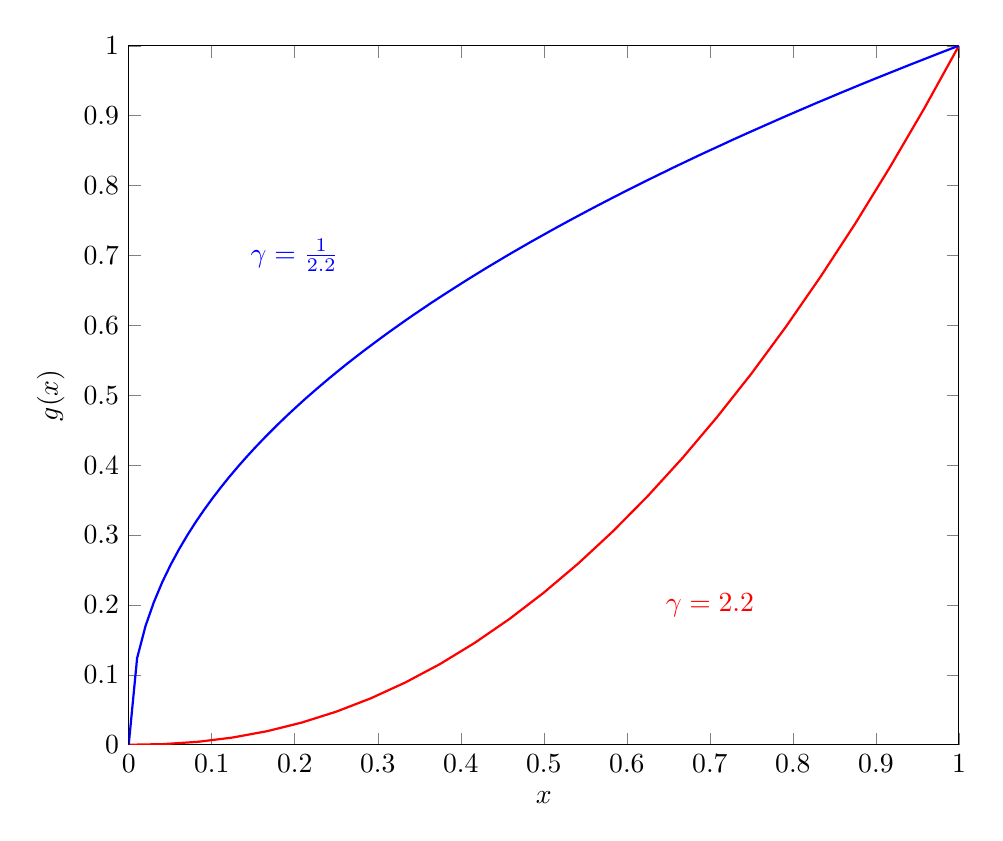
\begin{tikzpicture}
\begin{axis}[xmin=0, xmax=1, ymin=0, ymax=1, width=\textwidth,
xlabel=$x$, ylabel=$g(x)$]
\addplot[thick, red, domain=0:1] {x^2.2};
\node at (axis cs:0.2, 0.7) {\color{blue}$\gamma=\frac{1}{2.2}$};
\addplot[thick, blue, domain=0:1, samples=100] {x^0.4545};
\node at (axis cs:0.7, 0.2) {\color{red}$\gamma=2.2$};
\end{axis}
\end{tikzpicture}
\end{column}
\end{columns}
\end{frame}

\begin{frame}[c]{Gamma Correction -- Example}
    \begin{columns}[onlytextwidth]
        \begin{column}{0.30\textwidth}\centering
            \includegraphics[width=\textwidth]{img/brain_gamma0}\\ Gamma
            corrected $(\gamma=2.2)$
        \end{column}
        \begin{column}{0.30\textwidth}\centering
            \includegraphics[width=\textwidth]{img/brain}\\ Original
        \end{column}
        \begin{column}{0.30\textwidth}\centering
            \includegraphics[width=\textwidth]{img/brain_gamma1}\\ Gamma
            corrected $(\gamma=\frac{1}{2.2})$
        \end{column}
    \end{columns}
\end{frame}

\begin{frame}{Window and Level -- Example}
    \begin{columns}[T, onlytextwidth]
        \begin{column}{0.5\textwidth}\centering
            \includegraphics[height=0.75\textheight]{img/m1000-1000HU}

            $-1000$ HU to $1000$ HU
        \end{column}
        \begin{column}{0.5\textwidth}\centering
            \includegraphics[height=0.75\textheight]{img/200-500hu}

            $200$ HU to $500$ HU
        \end{column}
    \end{columns}
\end{frame}

\begin{frame}
    \frametitle{Histograms of Images}
    Histograms show the distribution of intensity values, grouped into
    \emph{bins}.
    \bigskip
    %	\tikzsetnextfilename{lenahist256}
    %		\begin{tikzpicture}
    %\end{tikzpicture}
    %	\tikzsetnextfilename{lenahist16}
    %		\begin{tikzpicture}
    %		\end{tikzpicture}

    \begin{columns}[T, onlytextwidth]
        \begin{column}{0.475\textwidth}\centering
            \tikzsetnextfilename{lenahist256}
            \begin{tikzpicture}[scale=0.9]
                \begin{axis}[width=\textwidth, height=0.8\textwidth, title={$256$ bins},
                        xtick={0,64,...,256}, xmin=0, xmax=255, ymin=0, xlabel=Intensity,
                        ylabel={$n_i$}, ylabel style={yshift=0.25em}]
                    \addplot[ybar, bar width=0.5, draw=none, fill=faublue!60!white] table[header=false,col sep=comma]
                        {img/lena_hist256.dat};
                \end{axis}
            \end{tikzpicture}
        \end{column}
        \begin{column}{0.475\textwidth}\centering
            \tikzsetnextfilename{lenahist16}
            \begin{tikzpicture}[scale=0.9]
                \begin{axis}[width=\textwidth, height=0.8\textwidth, ylabel
                    style={yshift=0.75em}, xmax=15, xtick={0, 4, 8, 12, 16}, xticklabels={0,
                            64, 128, 192, 256}, scaled ticks=false, title={$16$ bins}, xmin=0, ymin=0, xlabel=Intensity,
                    ylabel={$n_i$}]
                    \addplot[ybar, bar width=7.8, draw=none, fill=faublue!60!white] table[header=false,col sep=comma]
                        {img/lena_hist16.dat};
                \end{axis}
            \end{tikzpicture}
        \end{column}
    \end{columns}
\end{frame}



\begin{frame}
    \frametitle{Histogram Equalization}
    Intensities occupy only a small range in the histogram
    \bigskip

    \begin{columns}[c, onlytextwidth]
        \begin{column}{0.5\textwidth}\centering
            \includegraphics[height=0.7\textheight]{img/lena_bw}
        \end{column}%
        \begin{column}{0.5\textwidth}\centering
            \begin{tikzpicture}
                \begin{axis}[width=0.9\textwidth, height=0.8\textwidth, scaled ticks=false, ytick={0, 0.005, 0.01, 0.015}, yticklabels={0, 0.005, 0.010,
                                0.015}, xlabel=Intensity, ylabel={$n_i$}, xtick={0,64,...,256}, xmin=0, xmax=255, ymin=0]
                    %\addplot[lmehist, fill=faublue!60!white,
                    %draw=faublue] table {img/lena.dat};
                    \addplot[ybar, bar width=0.5, draw=none, fill=faublue!60!white] table[header=false,col sep=comma]
                        {img/lena_hist_norm256.dat};
                \end{axis}
            \end{tikzpicture}%
        \end{column}
    \end{columns}
\end{frame}


\begin{frame}
    \frametitle{Histogram Equalization}
    \begin{block}{Goal of Histogram Equalization}
        Achieve a uniform distribution of intensities $\Rightarrow$ \textbf{linear CDF}
    \end{block}
    \bigskip

    \begin{columns}[c, onlytextwidth]
        \begin{column}{0.475\textwidth}\centering
            \begin{tikzpicture}
                \begin{axis}[intaxis, width=0.9\textwidth, height=0.8\textwidth,
                        ylabel={$cdf(i)$}, ymax=1]
                    \addplot[faublue!80!white] table[header=false, col sep=comma]
                        {img/lena_cfd256.dat};
                \end{axis}
            \end{tikzpicture}
        \end{column}
        \begin{column}{0.05\textwidth}
            $\boldsymbol{\Rightarrow}$
        \end{column}
        \begin{column}{0.475\textwidth}\centering
            \begin{tikzpicture}
                \begin{axis}[intaxis, width=0.9\textwidth, height=0.8\textwidth,
                        ylabel={$cdf(i)$}, ymax=1]
                    \addplot[faublue!80!white] table[header=false, col sep=comma]
                        {img/lena_eq_cfd256.dat};
                \end{axis}
            \end{tikzpicture}
        \end{column}
    \end{columns}
\end{frame}

\begin{frame}
    \frametitle{Histogram Equalization}
    The histogram may contain gaps after histogram equalization!
    \bigskip

    \begin{columns}[c, onlytextwidth]
        \begin{column}{0.5\textwidth}\centering
            \includegraphics[height=0.7\textheight]{img/lena_histeq}
        \end{column}%
        \begin{column}{0.5\textwidth}\centering
            \begin{tikzpicture}
                \begin{axis}[width=0.9\textwidth, height=0.8\textwidth, scaled ticks=false, ytick={0, 0.005, 0.01, 0.015}, yticklabels={0, 0.005, 0.010,
                                0.015}, xlabel=Intensity, ylabel={$n_i$}, xtick={0,64,...,256}, xmin=0, xmax=255, ymin=0]
                    %\addplot[lmehist, fill=faublue!60!white,
                    %draw=faublue] table {img/lena.dat};
                    \addplot[ybar, bar width=0.5, draw=none, fill=faublue!60!white] table[header=false,col sep=comma]
                        {img/lena_eq_hist256.dat};
                \end{axis}
            \end{tikzpicture}%
        \end{column}
    \end{columns}
\end{frame}


\begin{frame}
    \frametitle{Histogram Equalization}
    \begin{columns}[T, onlytextwidth]
        \begin{column}{0.5\textwidth}\centering
            \includegraphics[height=0.7\textheight]{img/lena_bw}

            Before
        \end{column}
        \begin{column}{0.5\textwidth}\centering
            \includegraphics[height=0.7\textheight]{img/lena_histeq}

            After
        \end{column}
    \end{columns}
\end{frame}


\begin{frame}
    \frametitle{Demo}
    Demo in ImageJ \url{https://imagej.nih.gov/ij/} and MITK \url{mitk.org}
    \bigskip
\end{frame}


% TODO: change to calculate convolution not correlation
\begin{frame}
    \frametitle{Derivatives of Images}
    \begin{block}{Continuous derivative}
        \begin{equation*}
            f'(x) = \lim_{h\rightarrow0}\frac{f(x+h)-f(x)}{h}
        \end{equation*}
    \end{block}
    \begin{block}{Discrete derivatives}
        Several choices:

        \begin{center}
            \begin{tabularx}{0.8\textwidth}{lX}
                forward difference                    & $\Delta_x f(x) = f(x+1) - f(x)$   \\
                \rule{0pt}{1.5em}central difference   & $\delta_x f(x) = f(x+1) - f(x-1)$ \\
                \rule{0pt}{1.5em}backwards difference & $\nabla_x f(x) = f(x) - f(x-1)$
            \end{tabularx}
        \end{center}
    \end{block}
\end{frame}

\begin{frame}
    \frametitle{Derivatives of Images -- Example}
    \begin{columns}[T, onlytextwidth]
        \begin{column}{0.5\textwidth}\centering
            \includegraphics[height=0.7\textheight]{img/lena_dx}

            Derivative in $x$-direction
        \end{column}
        \begin{column}{0.5\textwidth}\centering
            \includegraphics[height=0.7\textheight]{img/lena_dy}

            Derivative in $y$-direction
        \end{column}
    \end{columns}
\end{frame}

\begin{frame}
    \frametitle{Image Filtering}
    \begin{block}{Filters as operators}
        A filter $\mathcal{H}$ can be applied on an image $f$:
        \begin{center}
            $\mathcal{H}(f(x,y)) = r(x,y)$
        \end{center}
        It can have the same properties as in 1-D:
        \bigskip

        \begin{tabularx}{\textwidth}{lX}
            \multirow{2}{*}{linearity} & \rule{0pt}{1.25em}$\mathcal{H}\lbrace\alpha\cdot f(x,y)\rbrace = \alpha\cdot
                \mathcal{H}\lbrace f(x,y)\rbrace$                                                                              \\
                                       & \rule{0pt}{1.25em}$\mathcal{H}\lbrace f_1(x,y) + f_2(x,y)\rbrace = \mathcal{H}\lbrace
                f_1(x,y)\rbrace + \mathcal{H}\lbrace f_2(x,y)\rbrace$                                                          \\
            shift-invariance           & \rule{0pt}{2em}$\mathcal{H}\lbrace (f(x-x_0, y-y_0)\rbrace = r(x-x_0, y-y_0)$
        \end{tabularx}
    \end{block}
\end{frame}

\begin{frame}
    \frametitle{Linear, Shift-invariant Filters}
    \begin{block}{Filter kernels}
        Linear, shift-invariant filters are characterized by \textbf{filter kernels}
        $k$ and are applied to an image by a convolution.
    \end{block}
    \begin{block}{Convolution with a filter}
        Image $f$, filter kernel $k$\vspace{-0.5\bigskipamount}
        \begin{equation*}
            \mathcal{H}\lbrace f\rbrace(x,y) = f\ast k = \sum_{i=-\frac{w_k}{2}}^{\frac{w_k}{2}}
            \sum_{j=-\frac{h_k}{2}}^{\frac{h_k}{2}} f(x-i, y-j)\cdot k(i, j)
        \end{equation*}
    \end{block}\vspace{-0.5\bigskipamount}
\end{frame}

\begin{frame}
    \frametitle{Efficient Filtering}
    \begin{block}{Convolution in the Fourier domain}
        For large images and /  or filters:
        \begin{enumerate}
            \item Transform $f$ and $k$ to the Fourier domain
                  \begin{align*}
                      F & =	\mathcal{F}(f) & K & = \mathcal{F}(k)
                  \end{align*}
            \item Like in 1-D, convolution then is a simple multiplication
                  \begin{equation*}
                      \mathcal{F}\lbrace f\ast k\rbrace = F\cdot K
                  \end{equation*}
            \item Get the filtered image by transforming the result back to the
                  spatial domain
        \end{enumerate}
        % $\tilde{w}=\mathcal{F}(w),\, \tilde{g}=\mathcal{F}(g)$
        % \begin{equation*}
        %   \tilde{g}' = \underbrace{\tilde{w}\cdot\tilde{g}}_{\text{simple multiplication}}
        % \end{equation*}
    \end{block}

\end{frame}

\begin{frame}
	\frametitle{2-D Fourier Space}
	
	\begin{itemize}
		\item 2-D Fourier Space with phase patterns associated with some positions:
	\end{itemize}
	
	\vspace{-2ex}
	
	\begin{center}
		\input{tikz/k_space.tikz}
	\end{center}
\end{frame}


\begin{frame}
    \frametitle{Filter Kernel -- Example: Central Difference}
    Derivatives are usually calculated by applying a filter.
    \bigskip

    The kernel can be constructed from the corresponding equation:
    \bigskip

    \begin{center}
        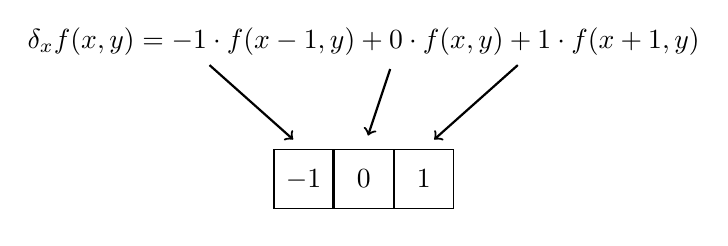
\begin{tikzpicture}
            \node[inner sep=0] (eq) {$\delta_xf(x,y) = -1\cdot f(x-1,y) +
                    0\cdot f(x,y)
                    +1\cdot f(x+1,y)$};
            \matrix (m) [below=3em of eq, filter kernel] {
                $-1$ \& $0$ \& $1$ \\
            };
            \draw[sarrow] (eq.185) to (m-1-1.north);
            \draw[sarrow] (eq.335) to (m-1-2.north);
            \draw[sarrow] (eq.355) to (m-1-3.north);
        \end{tikzpicture}
    \end{center}
\end{frame}

\begin{frame}
    \frametitle{Filter Kernels -- Derivative Filters}
    \begin{block}{First order derivatives}
        \hfill
        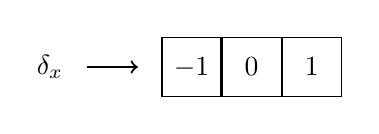
\begin{tikzpicture}[baseline=(current bounding box.center)]
            \matrix (m) [filter kernel] {
                $-1$ \& $0$ \& $1$ \\
            };
            \node [left= of m] (label) {$\delta_x$};
            \draw[sarrow] (label) to (m);
        \end{tikzpicture}\hfill
        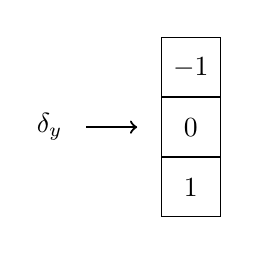
\begin{tikzpicture}[baseline=(current bounding box.center)]
            \matrix (m) [filter kernel] {
                $-1$ \\ $0$ \\ $1$\\
            };
            \node [left= of m] (label) {$\delta_y$};
            \draw[sarrow] (label) to (m);
        \end{tikzpicture}\hspace*{\fill}
    \end{block}
    \begin{block}{Second order derivative}
        \hspace*{\fill}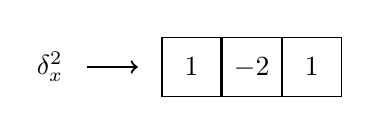
\begin{tikzpicture}[baseline=(current bounding box.center)]
            \matrix (m) [filter kernel] {
                $1$ \& $-2$ \& $1$ \\
            };
            \node [left= of m] (label) {$\delta^2_x$};
            \draw[sarrow] (label) to (m);
        \end{tikzpicture}\hspace*{\fill}
        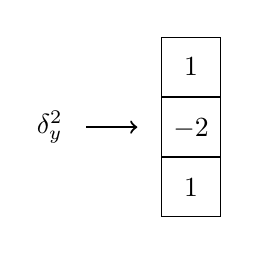
\begin{tikzpicture}[baseline=(current bounding box.center)]
            \matrix (m) [filter kernel] {
                $1$ \\ $-2$ \\ $1$\\
            };
            \node [left= of m] (label) {$\delta^2_y$};
            \draw[sarrow] (label) to (m);
        \end{tikzpicture}\hspace*{\fill}
    \end{block}
\end{frame}

\begin{frame}
    \frametitle{Smoothing Filters}
    Used to reduce noise in images.
    \begin{columns}[T, onlytextwidth]
        \begin{column}{0.45\textwidth}
            \begin{block}{Mean filter}\centering\bigskip\bigskip
                \includegraphics[width=0.5\textwidth]{images/mean}
            \end{block}
        \end{column}
        \begin{column}{0.45\textwidth}
            \begin{block}{Gaussian filter}\centering\bigskip\bigskip
                $\displaystyle\frac{1}{52}\,\cdot\,$ \raisebox{-0.28\textwidth}{\includegraphics[width=0.6\textwidth]{images/gauss}}
            \end{block}
        \end{column}
    \end{columns}
\end{frame}

\begin{frame}
    \frametitle{Gaussian Filtering}
    \begin{columns}[onlytextwidth]
        \begin{column}{0.5\textwidth}\centering
            \centering{}
            \includegraphics[height=0.8\textheight]{img/brain}\\Original
        \end{column}%
        \begin{column}{0.5\textwidth}\centering
            \centering{}
            \includegraphics[height=0.8\textheight]{img/brain_gauss}\\Blurred
        \end{column}
    \end{columns}
\end{frame}



\begin{frame}
	\frametitle{Derivative Filters and Noise}
	\includegraphics{img/lenadetailnoise}
	 \includegraphics{img/nonsobel}
	 \includegraphics{img/withsobel}
\end{frame}

%\begin{frame}
%  \frametitle{Derivatives of Images}
%  \begin{block}{Filters as derivatives}\bigskip
%        $\displaystyle\frac{\partial f}{\partial x} \quad\rightarrow\quad$\raisebox{-0.0175\textwidth}{\includegraphics[width=0.15\textwidth]{images/dy}}\qquad\qquad
%        $\displaystyle\frac{\partial f}{\partial y} \quad\rightarrow$\quad\raisebox{-0.068\textwidth}{\includegraphics[height=0.15\textwidth]{images/dx}}
%  \end{block}
%  \begin{block}{Sobel-Filter}
%    Combination with smoothing filter, less sensitive to noise\\\bigskip
%    $\displaystyle\frac{\partial f}{\partial x} \quad\rightarrow\quad\frac{1}{8}\,\cdot\,$\raisebox{-0.068\textwidth}{\includegraphics[width=0.15\textwidth]{images/sobel_x}}\qquad\qquad
%    $\displaystyle\frac{\partial f}{\partial x} \quad\rightarrow\quad\frac{1}{8}\,\cdot\,$\raisebox{-0.068\textwidth}{\includegraphics[width=0.15\textwidth]{images/sobel_y}}
%  \end{block}
%\end{frame}
%
%\begin{frame}
%  \frametitle{Derivatives of Images}
%  \begin{columns}[onlytextwidth]
%    \begin{column}{0.30\textwidth}\centering
%      \includegraphics[width=\textwidth]{images/brain}\\ Original
%    \end{column}
%    \begin{column}{0.30\textwidth}\centering
%      \includegraphics[width=\textwidth]{images/brain_sx}\\\medskip
%      $\displaystyle\frac{\partial}{\partial x}$\\\medskip vertical edges
%    \end{column}
%    \begin{column}{0.30\textwidth}\centering
%      \includegraphics[width=\textwidth]{images/brain_sy}\\\medskip
%      $\displaystyle\frac{\partial}{\partial y}$\\\medskip horizontal edges
%    \end{column}
%  \end{columns}
%\end{frame}

%\begin{frame}
%  \frametitle{Higher Order Derivatives}
%  \begin{block}{Laplace-Filter}
%    Laplace operator
%    \begin{equation*}
%      \Delta f(x,y)=\frac{\partial^2 f}{\partial x^2}+\frac{\partial^2
%        f}{\partial y^2}
%    \end{equation*}
%    As a filter
%    \begin{center}
%      $\displaystyle\Delta \quad\rightarrow\quad$\raisebox{-0.09\textwidth}{\includegraphics[width=0.21\textwidth]{images/laplacian}}
%    \end{center}
%  \end{block}
%\end{frame}

\subtitle{Image Processing -- Non-linear Methods}
\frame[plain,c]{\titlepage}

\begin{frame}[t]{Non-linear Filters}
    \begin{columns}[T, onlytextwidth]
        \begin{column}{0.4\textwidth}
            {\color{faublue}{\textbf{Median Filter}}}

            Rank ordering filter\bigskip
            \begin{enumerate}
                \item Sort intensities
                \item Choose value in the middle
            \end{enumerate}
        \end{column}%
        \begin{column}{0.5\textwidth}
            \raisebox{-0.1\textwidth}{\includegraphics[width=0.25\textwidth]{images/median_mask}}\quad%
            $\xrightarrow[\text{by value}]{\text{sort}}$\quad%
            \raisebox{-0.65\textwidth}{\includegraphics[width=0.08\textwidth]{images/median_vertical}}\quad%
            \raisebox{-0.31\textwidth}{$\xleftarrow{\text{median}}$}
        \end{column}
    \end{columns}
    \vspace{-4.5\bigskipamount}
    {\color{faublue}{\textbf{Differences to mean}}}
    \begin{itemize}
        \item Good against salt and pepper noise
        \item More robust against outliers
              %        \item not separable, higher computational cost
    \end{itemize}
\end{frame}

\begin{frame}[c]{Median Filtering}
    \begin{columns}[c,onlytextwidth]
        \begin{column}{0.45\textwidth}\centering
            \begin{figure}[]
                \centering
                \includegraphics[width=0.9\textwidth]{img/lena_sp}
                \caption{Original corrupted with noise}%
                \label{fig:name}
            \end{figure}
            %\includegraphics[width=0.9\textwidth]{img/lena_sp}\\Original\\corrupted
            %with noise
        \end{column}
        \begin{column}{0.45\textwidth}\centering
            \begin{figure}[]
                \centering
                \includegraphics[width=0.9\textwidth]{img/lena_sp_median}
                \caption{Median filtered}%
                \label{fig:name}
            \end{figure}
        \end{column}
    \end{columns}
\end{frame}

\begin{frame}[c]{Segmentation}
    \begin{block}{Goal}
        Separation of regions in images:
        \begin{itemize}
            \item Organs
            \item Bones
        \end{itemize}
    \end{block}
    \begin{block}{Thresholding}
        Image $f$, segmented image $t$, threshold $\theta$
        \begin{equation*}
            t(x,y) =
            \begin{cases}
                1 & \mbox{if } f(x,y)\geq \theta \\
                0 & \mbox{otherwise}
            \end{cases}
        \end{equation*}
    \end{block}
\end{frame}

\begin{frame}[c]{Segmentation}
    \begin{columns}[onlytextwidth,T]
        \begin{column}{0.475\textwidth}
            \begin{block}{How to choose $\theta$?}
                \begin{itemize}
                    \item manual by visual inspection
                    \item For bimodal histograms:
                          \begin{itemize}
                              \item Intersection of Gaussians
                              \item Otsu's method
                          \end{itemize}
                \end{itemize}
            \end{block}
        \end{column}
        \begin{column}{0.475\textwidth}
            \centering
            \tikzsetnextfilename{seghist256}
            \begin{tikzpicture}
                \begin{axis}[intaxis, ylabel={$n_i$}, width=\textwidth, height=0.6\textwidth, ylabel
                    style={yshift=+0.5em}, scaled ticks=false]
                    \addplot[ybar, bar width=0.5, draw=none, fill=faublue!60!white] table[header=false,col sep=comma]
                        {img/seg_circles.dat};
                    %				\draw[red, thick] (134, 0) -- (134,10000);
                \end{axis}
            \end{tikzpicture}
            Bimodal histogram
        \end{column}
    \end{columns}
\end{frame}

\begin{frame}{Segmentation -- Manual thresholds}
    \vspace{-0.5em}
    \begin{columns}[onlytextwidth,T]
        \begin{column}{0.32\textwidth}
            \centering{}
            \includegraphics[height=0.5\textheight]{img/brain.png}
            \\[0.5em]
            \begin{tikzpicture}[scale=0.73]
                \begin{axis}[intaxis, ylabel={$n_i$}, width=0.95\textwidth, height=.9\textwidth, ylabel
                    style={yshift=+0.5em}, xtick={0, 128, 255}, ytick={5e3, 15e3}, ymax=20000, scaled ticks=false]
                    \addplot[ybar, bar width=0.5, draw=none, fill=faublue!60!white] table[header=false,col sep=comma]
                        {img/brain_hist.dat};
                \end{axis}
                %\draw[rectangle] at (current bounding box);
            \end{tikzpicture}
        \end{column}%
        \begin{column}{0.32\textwidth}
            \centering{}
            \includegraphics[height=0.5\textheight]{img/brain_t50.png}
            \\[0.5em]
            \begin{tikzpicture}[scale=0.73]
                \begin{axis}[intaxis, ylabel={$n_i$}, width=0.95\textwidth, height=0.9\textwidth, ylabel
                    style={yshift=+0.5em}, xtick={0, 128, 255}, ytick={5e3, 15e3}, ymax=20000, scaled ticks=false]
                    \addplot[ybar, bar width=0.5, draw=none, fill=faublue!60!white] table[header=false,col sep=comma]
                        {img/brain_hist.dat};
                    \draw[red, thick] (50, 0) -- (50,10000);
                \end{axis}
            \end{tikzpicture}
        \end{column}
        \begin{column}{0.32\textwidth}
            \centering{}
            \includegraphics[height=0.5\textheight]{img/brain_t200.png}
            \\[0.5em]
            \begin{tikzpicture}[scale=0.73]
                \begin{axis}[intaxis, ylabel={$n_i$}, width=0.95\textwidth, height=0.9\textwidth, ylabel
                    style={yshift=+0.5em}, xtick={0, 128, 255}, ytick={5e3, 15e3}, ymax=20000, scaled ticks=false]
                    \addplot[ybar, bar width=0.5, draw=none, fill=faublue!60!white] table[header=false,col sep=comma]
                        {img/brain_hist.dat};
                    \draw[red, thick] (200, 0) -- (200,10000);
                \end{axis}
            \end{tikzpicture}
        \end{column}
    \end{columns}
\end{frame}

\begin{frame}{Segmentation -- Otsu's Method}
    \begin{columns}[onlytextwidth,c]
        \begin{column}{0.475\textwidth}
            \centering
            \includegraphics[height=0.4\textheight]{img/seg_circles_noise}
        \end{column}%
        \begin{column}{0.475\textwidth}
            \hspace{-1cm}
            \begin{tikzpicture}[scale=0.85]
                \begin{axis}[intaxis, ylabel={$n_i$}, width=\textwidth, height=0.6\textwidth, ylabel
                    style={yshift=+0.5em}, scaled ticks=false]
                    \addplot[ybar, bar width=0.5, draw=none, fill=faublue!60!white] table[header=false,col sep=comma]
                        {img/seg_circles.dat};
                \end{axis}
            \end{tikzpicture}
        \end{column}
    \end{columns}
    \vspace{1em}
    \begin{columns}[onlytextwidth,c]
        \begin{column}{0.475\textwidth}
            \centering
            \includegraphics[height=0.4\textheight]{img/seg_circles_seg}
        \end{column}\begin{column}{0.475\textwidth}
            \hspace{-1cm}
            \begin{tikzpicture}[scale=0.85]
                \begin{axis}[intaxis, ylabel={$n_i$}, width=\textwidth, height=0.6\textwidth, ylabel
                    style={yshift=+0.5em}, scaled ticks=false]
                    \addplot[ybar, bar width=0.5, draw=none, fill=faublue!60!white] table[header=false,col sep=comma]
                        {img/seg_circles.dat};
                    \draw[red, thick] (134, 0) -- (134,10000);
                \end{axis}
            \end{tikzpicture}
        \end{column}
    \end{columns}
\end{frame}

\begin{frame}{Morphological Operations}
    \begin{block}{Treat image as set of tuples $(x,y,f(x,y))$}
        \begin{equation*}
            \mathrm{F} = \Big\lbrace\big(x_0, y_0, f(x_0, y_0)\big),\, \big(x_1, y_1, f(x_1,
            y_1)\big),\, \ldots,\, \big(x_n,
            y_n, f(x_n, y_n)\big)\Big\rbrace\,.
        \end{equation*}
    \end{block}
    \begin{block}{Morphological operator}
        \begin{itemize}
            \item structuring element $\mathrm{S}_{(x,y)}$
            \item operation
        \end{itemize}
    \end{block}
\end{frame}

\begin{frame}
    \frametitle{Morphological Operations}
    \begin{block}{Structuring element $\mathrm{S}_{(x,y)}$}
        ``Kernel'' of the morphological operation
    \end{block}

    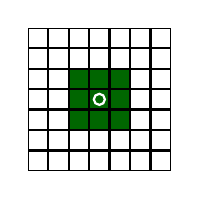
\begin{tikzpicture}
        \matrix (sel) [se] {
            \node[bg] {}; \& \node[bg] {}; \& \node[bg] {}; \& \node[bg] {}; \& \node[bg] {}; \& \node[bg] {}; \& \node[bg] {}; \& \\
            \node[bg] {}; \& \node[bg] {}; \& \node[bg] {}; \& \node[bg] {}; \& \node[bg] {}; \& \node[bg] {}; \& \node[bg] {}; \& \\
            \node[bg] {}; \& \node[bg] {}; \& \node[fgse] {}; \& \node[fgse] {}; \& \node[fgse] {}; \& \node[bg] {}; \& \node[bg] {}; \& \\
            \node[bg] {}; \& \node[bg] {}; \& \node[fgse] {}; \& \node[fgse] (c) {}; \& \node[fgse] {}; \& \node[bg] {}; \& \node[bg] {}; \& \\
            \node[bg] {}; \& \node[bg] {}; \& \node[fgse] {}; \& \node[fgse] {}; \& \node[fgse] {}; \& \node[bg] {}; \& \node[bg] {}; \& \\
            \node[bg] {}; \& \node[bg] {}; \& \node[bg] {}; \& \node[bg] {}; \& \node[bg] {}; \& \node[bg] {}; \& \node[bg] {}; \& \\
            \node[bg] {}; \& \node[bg] {}; \& \node[bg] {}; \& \node[bg] {}; \& \node[bg] {}; \& \node[bg] {}; \& \node[bg] {}; \& \\
        };
        \node[draw=white, circle, inner sep=0, minimum width=0.4em, thick] at	(c.center) {};
    \end{tikzpicture}
    \tikzsetnextfilename{selcross}
    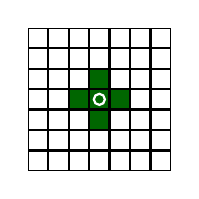
\begin{tikzpicture}
        \matrix (sel) [se] {
            \node[bg] {}; \& \node[bg] {}; \& \node[bg] {}; \& \node[bg] {}; \& \node[bg] {}; \& \node[bg] {}; \& \node[bg] {}; \& \\
            \node[bg] {}; \& \node[bg] {}; \& \node[bg] {}; \& \node[bg] {}; \& \node[bg] {}; \& \node[bg] {}; \& \node[bg] {}; \& \\
            \node[bg] {}; \& \node[bg] {}; \& \node[bg] {}; \& \node[fgse] {}; \& \node[bg] {}; \& \node[bg] {}; \& \node[bg] {}; \& \\
            \node[bg] {}; \& \node[bg] {}; \& \node[fgse] {}; \& \node[fgse] (c) {}; \& \node[fgse] {}; \& \node[bg] {}; \& \node[bg] {}; \& \\
            \node[bg] {}; \& \node[bg] {}; \& \node[bg] {}; \& \node[fgse] {}; \& \node[bg] {}; \& \node[bg] {}; \& \node[bg] {}; \& \\
            \node[bg] {}; \& \node[bg] {}; \& \node[bg] {}; \& \node[bg] {}; \& \node[bg] {}; \& \node[bg] {}; \& \node[bg] {}; \& \\
            \node[bg] {}; \& \node[bg] {}; \& \node[bg] {}; \& \node[bg] {}; \& \node[bg] {}; \& \node[bg] {}; \& \node[bg] {}; \& \\
        };
        \node[draw=white, circle, inner sep=0, minimum width=0.4em, thick] at	(c.center) {};
    \end{tikzpicture}
    \tikzsetnextfilename{seldiamond}
    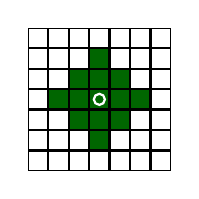
\begin{tikzpicture}
        \matrix (sel) [se] {
            \node[bg] {}; \& \node[bg] {}; \& \node[bg] {}; \& \node[bg] {}; \& \node[bg] {}; \& \node[bg] {}; \& \node[bg] {}; \& \\
            \node[bg] {}; \& \node[bg] {}; \& \node[bg] {}; \& \node[fgse] {}; \& \node[bg] {}; \& \node[bg] {}; \& \node[bg] {}; \& \\
            \node[bg] {}; \& \node[bg] {}; \& \node[fgse] {}; \& \node[fgse] {}; \& \node[fgse] {}; \& \node[bg] {}; \& \node[bg] {}; \& \\
            \node[bg] {}; \& \node[fgse] {}; \& \node[fgse] {}; \& \node[fgse] (c) {}; \& \node[fgse] {}; \& \node[fgse] {}; \& \node[bg] {}; \& \\
            \node[bg] {}; \& \node[bg] {}; \& \node[fgse] {}; \& \node[fgse] {}; \& \node[fgse] {}; \& \node[bg] {}; \& \node[bg] {}; \& \\
            \node[bg] {}; \& \node[bg] {}; \& \node[bg] {}; \& \node[fgse] {}; \& \node[bg] {}; \& \node[bg] {}; \& \node[bg] {}; \& \\
            \node[bg] {}; \& \node[bg] {}; \& \node[bg] {}; \& \node[bg] {}; \& \node[bg] {}; \& \node[bg] {}; \& \node[bg] {}; \& \\
        };
        \node[draw=white, circle, inner sep=0, minimum width=0.4em, thick] at	(c.center) {};
    \end{tikzpicture}
    \tikzsetnextfilename{selbar}
    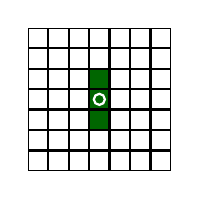
\begin{tikzpicture}
        \matrix (sel) [se] {
            \node[bg] {}; \& \node[bg] {}; \& \node[bg] {}; \& \node[bg] {}; \& \node[bg] {}; \& \node[bg] {}; \& \node[bg] {}; \& \\
            \node[bg] {}; \& \node[bg] {}; \& \node[bg] {}; \& \node[bg] {}; \& \node[bg] {}; \& \node[bg] {}; \& \node[bg] {}; \& \\
            \node[bg] {}; \& \node[bg] {}; \& \node[bg] {}; \& \node[fgse] {}; \& \node[bg] {}; \& \node[bg] {}; \& \node[bg] {}; \& \\
            \node[bg] {}; \& \node[bg] {}; \& \node[bg] {}; \& \node[fgse] (c) {}; \& \node[bg] {}; \& \node[bg] {}; \& \node[bg] {}; \& \\
            \node[bg] {}; \& \node[bg] {}; \& \node[bg] {}; \& \node[fgse] {}; \& \node[bg] {}; \& \node[bg] {}; \& \node[bg] {}; \& \\
            \node[bg] {}; \& \node[bg] {}; \& \node[bg] {}; \& \node[bg] {}; \& \node[bg] {}; \& \node[bg] {}; \& \node[bg] {}; \& \\
            \node[bg] {}; \& \node[bg] {}; \& \node[bg] {}; \& \node[bg] {}; \& \node[bg] {}; \& \node[bg] {}; \& \node[bg] {}; \& \\
        };
        \node[draw=white, circle, inner sep=0, minimum width=0.4em, thick] at	(c.center) {};
    \end{tikzpicture}
    \tikzsetnextfilename{selL}
    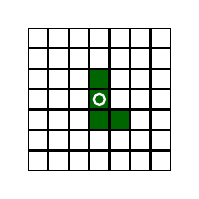
\begin{tikzpicture}
        \matrix (sel) [se] {
            \node[bg] {}; \& \node[bg] {}; \& \node[bg] {}; \& \node[bg] {}; \& \node[bg] {}; \& \node[bg] {}; \& \node[bg] {}; \& \\
            \node[bg] {}; \& \node[bg] {}; \& \node[bg] {}; \& \node[bg] {}; \& \node[bg] {}; \& \node[bg] {}; \& \node[bg] {}; \& \\
            \node[bg] {}; \& \node[bg] {}; \& \node[bg] {}; \& \node[fgse] {}; \& \node[bg] {}; \& \node[bg] {}; \& \node[bg] {}; \& \\
            \node[bg] {}; \& \node[bg] {}; \& \node[bg] {}; \& \node[fgse] (c) {}; \& \node[bg] {}; \& \node[bg] {}; \& \node[bg] {}; \& \\
            \node[bg] {}; \& \node[bg] {}; \& \node[bg] {}; \& \node[fgse] {}; \& \node[fgse] {}; \& \node[bg] {}; \& \node[bg] {}; \& \\
            \node[bg] {}; \& \node[bg] {}; \& \node[bg] {}; \& \node[bg] {}; \& \node[bg] {}; \& \node[bg] {}; \& \node[bg] {}; \& \\
            \node[bg] {}; \& \node[bg] {}; \& \node[bg] {}; \& \node[bg] {}; \& \node[bg] {}; \& \node[bg] {}; \& \node[bg] {}; \& \\
        };
        \node[draw=white, circle, inner sep=0, minimum width=0.4em, thick] at	(c.center) {};
    \end{tikzpicture}
\end{frame}

\begin{frame}{Morphological Operations}
    \begin{block}{Binary erosion}
        \begin{equation*}
            \mathrm{F} \ominus \mathrm{S} = \big\lbrace(x,y) : \mathrm{S}_{(x,y)}\subset
            \mathrm{F} \big\rbrace\,.
        \end{equation*}
    \end{block}
    \begin{center}
        \tikzsetnextfilename{morphinput}
        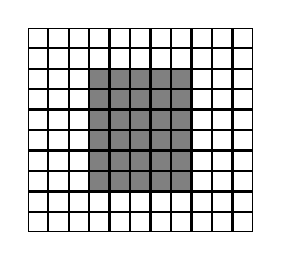
\begin{tikzpicture}[baseline={([yshift=-0.5ex]current bounding box.center)}]
            \matrix (img) [se] {
                \node[bg] {}; \& \node[bg] {}; \& \node[bg] {}; \& \node[bg] {}; \&	\node[bg] {}; \& \node[bg] {}; \& \node[bg] {}; \& \node[bg] {}; \&	\node[bg] {}; \& \node[bg] {}; \& \node[bg] {}; \\
                \node[bg] {}; \& \node[bg] {}; \& \node[bg] {}; \& \node[bg] {}; \&	\node[bg] {}; \& \node[bg] {}; \& \node[bg] {}; \& \node[bg] {}; \&	\node[bg] {}; \& \node[bg] {}; \& \node[bg] {}; \\
                \node[bg] {}; \& \node[bg] {}; \& \node[bg] {}; \& \node[fg] {}; \&	\node[fg] {}; \& \node[fg] {}; \& \node[fg] {}; \& \node[fg] {}; \&	\node[bg] {}; \& \node[bg] {}; \& \node[bg] {}; \\
                \node[bg] {}; \& \node[bg] {}; \& \node[bg] {}; \& \node[fg] {}; \&	\node[fg] {}; \& \node[fg] {}; \& \node[fg] {}; \& \node[fg] {}; \&	\node[bg] {}; \& \node[bg] {}; \& \node[bg] {}; \\
                \node[bg] {}; \& \node[bg] {}; \& \node[bg] {}; \& \node[fg] {}; \&	\node[fg] {}; \& \node[fg] {}; \& \node[fg] {}; \& \node[fg] {}; \&	\node[bg] {}; \& \node[bg] {}; \& \node[bg] {}; \\
                \node[bg] {}; \& \node[bg] {}; \& \node[bg] {}; \& \node[fg] {}; \&	\node[fg] {}; \& \node[fg] {}; \& \node[fg] {}; \& \node[fg] {}; \&	\node[bg] {}; \& \node[bg] {}; \& \node[bg] {}; \\
                \node[bg] {}; \& \node[bg] {}; \& \node[bg] {}; \& \node[fg] {}; \&	\node[fg] {}; \& \node[fg] {}; \& \node[fg] {}; \& \node[fg] {}; \&	\node[bg] {}; \& \node[bg] {}; \& \node[bg] {}; \\
                \node[bg] {}; \& \node[bg] {}; \& \node[bg] {}; \& \node[fg] {}; \&	\node[fg] {}; \& \node[fg] {}; \& \node[fg] {}; \& \node[fg] {}; \&	\node[bg] {}; \& \node[bg] {}; \& \node[bg] {}; \\
                \node[bg] {}; \& \node[bg] {}; \& \node[bg] {}; \& \node[bg] {}; \&	\node[bg] {}; \& \node[bg] {}; \& \node[bg] {}; \& \node[bg] {}; \&	\node[bg] {}; \& \node[bg] {}; \& \node[bg] {}; \\
                \node[bg] {}; \& \node[bg] {}; \& \node[bg] {}; \& \node[bg] {}; \&	\node[bg] {}; \& \node[bg] {}; \& \node[bg] {}; \& \node[bg] {}; \&	\node[bg] {}; \& \node[bg] {}; \& \node[bg] {}; \\
            };
        \end{tikzpicture}
        $\rightarrow$
        \tikzsetnextfilename{erosion1}
        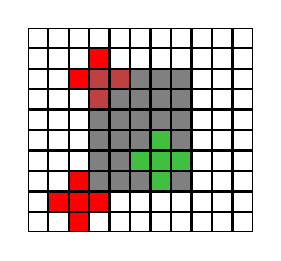
\begin{tikzpicture}[baseline={([yshift=-0.5ex]current bounding box.center)}]
            \matrix (img) [se] {
                \node[bg] {}; \& \node[bg] {}; \& \node[bg] {}; \& \node[bg] {}; \&	\node[bg] {}; \& \node[bg] {}; \& \node[bg] {}; \& \node[bg] {}; \&	\node[bg] {}; \& \node[bg] {}; \& \node[bg] {}; \\
                \node[bg] {}; \& \node[bg] {}; \& \node[bg] {}; \& \node[sen] {}; \&	\node[bg] {}; \& \node[bg] {}; \& \node[bg] {}; \& \node[bg] {}; \&	\node[bg] {}; \& \node[bg] {}; \& \node[bg] {}; \\
                \node[bg] {}; \& \node[bg] {}; \& \node[sen] {}; \& \node[senm] {}; \&	\node[senm] {}; \& \node[fg] {}; \& \node[fg] {}; \& \node[fg] {}; \&	\node[bg] {}; \& \node[bg] {}; \& \node[bg] {}; \\
                \node[bg] {}; \& \node[bg] {}; \& \node[bg] {}; \& \node[senm] {}; \&	\node[fg] {}; \& \node[fg] {}; \& \node[fg] {}; \& \node[fg] {}; \&	\node[bg] {}; \& \node[bg] {}; \& \node[bg] {}; \\
                \node[bg] {}; \& \node[bg] {}; \& \node[bg] {}; \& \node[fg] {}; \&	\node[fg] {}; \& \node[fg] {}; \& \node[fg] {}; \& \node[fg] {}; \&	\node[bg] {}; \& \node[bg] {}; \& \node[bg] {}; \\
                \node[bg] {}; \& \node[bg] {}; \& \node[bg] {}; \& \node[fg] {}; \&	\node[fg] {}; \& \node[fg] {}; \& \node[sepm] {}; \& \node[fg] {}; \&	\node[bg] {}; \& \node[bg] {}; \& \node[bg] {}; \\
                \node[bg] {}; \& \node[bg] {}; \& \node[bg] {}; \& \node[fg] {}; \&	\node[fg] {}; \& \node[sepm] {}; \& \node[sepm] {}; \& \node[sepm] {}; \&	\node[bg] {}; \& \node[bg] {}; \& \node[bg] {}; \\
                \node[bg] {}; \& \node[bg] {}; \& \node[sen] {}; \& \node[fg] {}; \&	\node[fg] {}; \& \node[fg] {}; \& \node[sepm] {}; \& \node[fg] {}; \&	\node[bg] {}; \& \node[bg] {}; \& \node[bg] {}; \\
                \node[bg] {}; \& \node[sen] {}; \& \node[sen] {}; \& \node[sen] {}; \&	\node[bg] {}; \& \node[bg] {}; \& \node[bg] {}; \& \node[bg] {}; \&	\node[bg] {}; \& \node[bg] {}; \& \node[bg] {}; \\
                \node[bg] {}; \& \node[bg] {}; \& \node[sen] {}; \& \node[bg] {}; \&	\node[bg] {}; \& \node[bg] {}; \& \node[bg] {}; \& \node[bg] {}; \&	\node[bg] {}; \& \node[bg] {}; \& \node[bg] {}; \\
            };
        \end{tikzpicture}
        $\rightarrow$
        \tikzsetnextfilename{erosion2}
        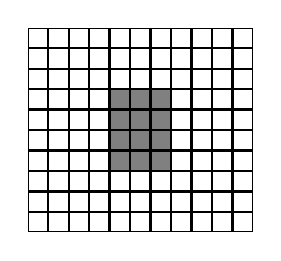
\begin{tikzpicture}[baseline={([yshift=-0.5ex]current bounding box.center)}]
            \matrix (img) [se] {
                \node[bg] {}; \& \node[bg] {}; \& \node[bg] {}; \& \node[bg] {}; \&	\node[bg] {}; \& \node[bg] {}; \& \node[bg] {}; \& \node[bg] {}; \&	\node[bg] {}; \& \node[bg] {}; \& \node[bg] {}; \\
                \node[bg] {}; \& \node[bg] {}; \& \node[bg] {}; \& \node[bg] {}; \&	\node[bg] {}; \& \node[bg] {}; \& \node[bg] {}; \& \node[bg] {}; \&	\node[bg] {}; \& \node[bg] {}; \& \node[bg] {}; \\
                \node[bg] {}; \& \node[bg] {}; \& \node[bg] {}; \& \node[bg] {}; \&	\node[bg] {}; \& \node[bg] {}; \& \node[bg] {}; \& \node[bg] {}; \&	\node[bg] {}; \& \node[bg] {}; \& \node[bg] {}; \\
                \node[bg] {}; \& \node[bg] {}; \& \node[bg] {}; \& \node[bg] {}; \&	\node[fg] {}; \& \node[fg] {}; \& \node[fg] {}; \& \node[bg] {}; \&	\node[bg] {}; \& \node[bg] {}; \& \node[bg] {}; \\
                \node[bg] {}; \& \node[bg] {}; \& \node[bg] {}; \& \node[bg] {}; \&	\node[fg] {}; \& \node[fg] {}; \& \node[fg] {}; \& \node[bg] {}; \&	\node[bg] {}; \& \node[bg] {}; \& \node[bg] {}; \\
                \node[bg] {}; \& \node[bg] {}; \& \node[bg] {}; \& \node[bg] {}; \&	\node[fg] {}; \& \node[fg] {}; \& \node[fg] {}; \& \node[bg] {}; \&	\node[bg] {}; \& \node[bg] {}; \& \node[bg] {}; \\
                \node[bg] {}; \& \node[bg] {}; \& \node[bg] {}; \& \node[bg] {}; \&	\node[fg] {}; \& \node[fg] {}; \& \node[fg] {}; \& \node[bg] {}; \&	\node[bg] {}; \& \node[bg] {}; \& \node[bg] {}; \\
                \node[bg] {}; \& \node[bg] {}; \& \node[bg] {}; \& \node[bg] {}; \&	\node[bg] {}; \& \node[bg] {}; \& \node[bg] {}; \& \node[bg] {}; \&	\node[bg] {}; \& \node[bg] {}; \& \node[bg] {}; \\
                \node[bg] {}; \& \node[bg] {}; \& \node[bg] {}; \& \node[bg] {}; \&	\node[bg] {}; \& \node[bg] {}; \& \node[bg] {}; \& \node[bg] {}; \&	\node[bg] {}; \& \node[bg] {}; \& \node[bg] {}; \\
                \node[bg] {}; \& \node[bg] {}; \& \node[bg] {}; \& \node[bg] {}; \&	\node[bg] {}; \& \node[bg] {}; \& \node[bg] {}; \& \node[bg] {}; \&	\node[bg] {}; \& \node[bg] {}; \& \node[bg] {}; \\
            };
        \end{tikzpicture}
    \end{center}
\end{frame}

\begin{frame}{Morphological Operations}
    \begin{block}{Binary dilation}
        \begin{equation*}
            \mathrm{F} \oplus \mathrm{S} = \big\lbrace (x,y): \mathrm{S}_{(x,y)} \cap
            \mathrm{F}\neq\emptyset\big\rbrace
        \end{equation*}
    \end{block}
    \begin{center}
        \tikzsetnextfilename{morphinput}
        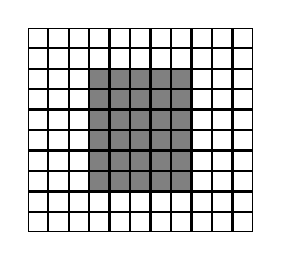
\begin{tikzpicture}[baseline={([yshift=-0.5ex]current bounding box.center)}]
            \matrix (img) [se] {
                \node[bg] {}; \& \node[bg] {}; \& \node[bg] {}; \& \node[bg] {}; \&	\node[bg] {}; \& \node[bg] {}; \& \node[bg] {}; \& \node[bg] {}; \&	\node[bg] {}; \& \node[bg] {}; \& \node[bg] {}; \\
                \node[bg] {}; \& \node[bg] {}; \& \node[bg] {}; \& \node[bg] {}; \&	\node[bg] {}; \& \node[bg] {}; \& \node[bg] {}; \& \node[bg] {}; \&	\node[bg] {}; \& \node[bg] {}; \& \node[bg] {}; \\
                \node[bg] {}; \& \node[bg] {}; \& \node[bg] {}; \& \node[fg] {}; \&	\node[fg] {}; \& \node[fg] {}; \& \node[fg] {}; \& \node[fg] {}; \&	\node[bg] {}; \& \node[bg] {}; \& \node[bg] {}; \\
                \node[bg] {}; \& \node[bg] {}; \& \node[bg] {}; \& \node[fg] {}; \&	\node[fg] {}; \& \node[fg] {}; \& \node[fg] {}; \& \node[fg] {}; \&	\node[bg] {}; \& \node[bg] {}; \& \node[bg] {}; \\
                \node[bg] {}; \& \node[bg] {}; \& \node[bg] {}; \& \node[fg] {}; \&	\node[fg] {}; \& \node[fg] {}; \& \node[fg] {}; \& \node[fg] {}; \&	\node[bg] {}; \& \node[bg] {}; \& \node[bg] {}; \\
                \node[bg] {}; \& \node[bg] {}; \& \node[bg] {}; \& \node[fg] {}; \&	\node[fg] {}; \& \node[fg] {}; \& \node[fg] {}; \& \node[fg] {}; \&	\node[bg] {}; \& \node[bg] {}; \& \node[bg] {}; \\
                \node[bg] {}; \& \node[bg] {}; \& \node[bg] {}; \& \node[fg] {}; \&	\node[fg] {}; \& \node[fg] {}; \& \node[fg] {}; \& \node[fg] {}; \&	\node[bg] {}; \& \node[bg] {}; \& \node[bg] {}; \\
                \node[bg] {}; \& \node[bg] {}; \& \node[bg] {}; \& \node[fg] {}; \&	\node[fg] {}; \& \node[fg] {}; \& \node[fg] {}; \& \node[fg] {}; \&	\node[bg] {}; \& \node[bg] {}; \& \node[bg] {}; \\
                \node[bg] {}; \& \node[bg] {}; \& \node[bg] {}; \& \node[bg] {}; \&	\node[bg] {}; \& \node[bg] {}; \& \node[bg] {}; \& \node[bg] {}; \&	\node[bg] {}; \& \node[bg] {}; \& \node[bg] {}; \\
                \node[bg] {}; \& \node[bg] {}; \& \node[bg] {}; \& \node[bg] {}; \&	\node[bg] {}; \& \node[bg] {}; \& \node[bg] {}; \& \node[bg] {}; \&	\node[bg] {}; \& \node[bg] {}; \& \node[bg] {}; \\
            };
        \end{tikzpicture}
        $\rightarrow$
        \tikzsetnextfilename{dilation}
        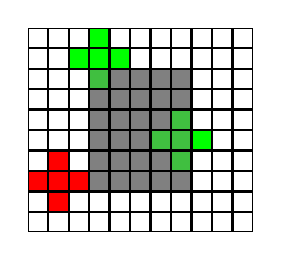
\begin{tikzpicture}[baseline={([yshift=-0.5ex]current bounding box.center)}]
            \matrix (img) [se] {
                \node[bg] {}; \& \node[bg] {}; \& \node[bg] {}; \& \node[sep] {}; \&	\node[bg] {}; \& \node[bg] {}; \& \node[bg] {}; \& \node[bg] {}; \&	\node[bg] {}; \& \node[bg] {}; \& \node[bg] {};  \\
                \node[bg] {}; \& \node[bg] {}; \& \node[sep] {}; \& \node[sep] {}; \&	\node[sep] {}; \& \node[bg] {}; \& \node[bg] {}; \& \node[bg] {}; \&	\node[bg] {}; \& \node[bg] {}; \& \node[bg] {};  \\
                \node[bg] {}; \& \node[bg] {}; \& \node[bg] {}; \& \node[sepm] {}; \&	\node[fg] {}; \& \node[fg] {}; \& \node[fg] {}; \& \node[fg] {}; \&	\node[bg] {}; \& \node[bg] {}; \& \node[bg] {};  \\
                \node[bg] {}; \& \node[bg] {}; \& \node[bg] {}; \& \node[fg] {}; \&	\node[fg] {}; \& \node[fg] {}; \& \node[fg] {}; \& \node[fg] {}; \&	\node[bg] {}; \& \node[bg] {}; \& \node[bg] {};  \\
                \node[bg] {}; \& \node[bg] {}; \& \node[bg] {}; \& \node[fg] {}; \&	\node[fg] {}; \& \node[fg] {}; \& \node[fg] {}; \& \node[sepm] {}; \&	\node[bg] {}; \& \node[bg] {}; \& \node[bg] {};  \\
                \node[bg] {}; \& \node[bg] {}; \& \node[bg] {}; \& \node[fg] {}; \&	\node[fg] {}; \& \node[fg] {}; \& \node[sepm] {}; \& \node[sepm] {}; \&	\node[sep] {}; \& \node[bg] {}; \& \node[bg] {};  \\
                \node[bg] {}; \& \node[sen] {}; \& \node[bg] {}; \& \node[fg] {}; \& \node[fg] {}; \& \node[fg] {}; \& \node[fg] {}; \& \node[sepm] {}; \&	\node[bg] {}; \& \node[bg] {}; \& \node[bg] {}; \\
                \node[sen] {}; \& \node[sen] {}; \& \node[sen] {}; \& \node[fg] {}; \&	\node[fg] {}; \& \node[fg] {}; \& \node[fg] {}; \& \node[fg] {}; \&	\node[bg] {}; \& \node[bg] {}; \& \node[bg] {};  \\
                \node[bg] {}; \& \node[sen] {}; \& \node[bg] {}; \& \node[bg] {}; \&	\node[bg] {}; \& \node[bg] {}; \& \node[bg] {}; \& \node[bg] {}; \&	\node[bg] {}; \& \node[bg] {}; \& \node[bg] {};  \\
                \node[bg] {}; \& \node[bg] {}; \& \node[bg] {}; \& \node[bg] {}; \&	\node[bg] {}; \& \node[bg] {}; \& \node[bg] {}; \& \node[bg] {}; \&	\node[bg] {}; \& \node[bg] {}; \& \node[bg] {};  \\
            };
        \end{tikzpicture}
        $\rightarrow$
        \tikzsetnextfilename{erosion2}
        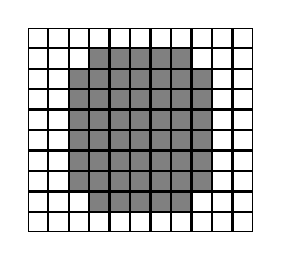
\begin{tikzpicture}[baseline={([yshift=-0.5ex]current bounding box.center)}]
            \matrix (img) [se] {
                \node[bg] {}; \& \node[bg] {}; \& \node[bg] {}; \& \node[bg] {}; \&	\node[bg] {}; \& \node[bg] {}; \& \node[bg] {}; \& \node[bg] {}; \&	\node[bg] {}; \& \node[bg] {}; \& \node[bg] {};            \\
                \node[bg] {}; \& \node[bg] {}; \& \node[bg] {}; \& \node[fg] {}; \&	\node[fg] {}; \& \node[fg] {}; \& \node[fg] {}; \& \node[fg] {}; \&	\node[bg] {}; \& \node[bg] {}; \& \node[bg] {};            \\
                \node[bg] {}; \& \node[bg] {}; \& \node[fg] {}; \& \node[fg] {}; \&	\node[fg] {}; \& \node[fg] {}; \& \node[fg] {}; \& \node[fg] {}; \&	\node[fg] {}; \& \node[bg] {}; \& \node[bg] {};            \\
                \node[bg] {}; \& \node[bg] {}; \& \node[fg] {}; \& \node[fg] {}; \&	\node[fg] {}; \& \node[fg] {}; \& \node[fg] {}; \& \node[fg] {}; \&	\node[fg] {}; \& \node[bg] {}; \& \node[bg] {};            \\
                \node[bg] {}; \& \node[bg] {}; \& \node[fg] {}; \& \node[fg] {}; \&	\node[fg] {}; \& \node[fg] {}; \& \node[fg] {}; \& \node[fg] {}; \&	\node[fg] {}; \& \node[bg] {}; \& \node[bg] {};            \\
                \node[bg] {}; \& \node[bg] {}; \& \node[fg] {}; \& \node[fg] {}; \&	\node[fg] {}; \& \node[fg] {}; \& \node[fg] {}; \& \node[fg] {}; \&	\node[fg] {}; \& \node[bg] {}; \& \node[bg] {};            \\
                \node[bg] {}; \& \node[bg] {}; \& \node[fg] {}; \& \node[fg] {}; \&	\node[fg] {}; \& \node[fg] {}; \& \node[fg] {}; \& \node[fg] {}; \&	\node[fg] {}; \& \node[bg] {}; \& \node[bg] {};     \\
                \node[bg] {}; \& \node[bg] {}; \& \node[fg] {}; \& \node[fg] {}; \&	\node[fg] {}; \& \node[fg] {}; \& \node[fg] {}; \& \node[fg] {}; \&	\node[fg] {}; \& \node[bg] {}; \& \node[bg] {}; \\
                \node[bg] {}; \& \node[bg] {}; \& \node[bg] {}; \& \node[fg] {}; \&	\node[fg] {}; \& \node[fg] {}; \& \node[fg] {}; \& \node[fg] {}; \&	\node[bg] {}; \& \node[bg] {}; \& \node[bg] {}; \\
                \node[bg] {}; \& \node[bg] {}; \& \node[bg] {}; \& \node[bg] {}; \&	\node[bg] {}; \& \node[bg] {}; \& \node[bg] {}; \& \node[bg] {}; \&	\node[bg] {}; \& \node[bg] {}; \& \node[bg] {}; \\
            };
        \end{tikzpicture}
    \end{center}
\end{frame}

\begin{frame}{Morphological Operations}
    \begin{block}{Grayscale versions}
        \begin{itemize}
            \item Erosion:
                  $(\mathrm{F}\ominus \mathrm{S})(x,y) = \min \big\lbrace \mathrm{S}_{(x,y)} \cap \mathrm{F}\big\rbrace$
            \item Dilation:
                  $(\mathrm{F}\oplus \mathrm{S})(x,y) = \max \big\lbrace \mathrm{S}_{(x,y)} \cap \mathrm{F}\big\rbrace$
        \end{itemize}
    \end{block}

    \begin{columns}[onlytextwidth,T]
        \begin{column}{0.3\textwidth}
            \centering{}
            \includegraphics[height=0.5\textheight]{img/lena_bw}

            Original
        \end{column}%
        \begin{column}{0.3\textwidth}
            \centering
            \includegraphics[height=0.5\textheight]{img/lena_er}

            Eroded image
        \end{column}%
        \begin{column}{0.3\textwidth}
            \centering
            \includegraphics[height=0.5\textheight]{img/lena_di}

            Dilated image
        \end{column}
    \end{columns}
\end{frame}

\begin{frame}
    \frametitle{Morphological Operations}
    \begin{block}{Opening}
        $\mathrm{F}\circ \mathrm{S} = (\mathrm{F}\ominus \mathrm{S})\oplus \mathrm{S} $
    \end{block}
    \begin{center}
        Erosion\\[0.1em]
        \raisebox{-0.07\textwidth}{
            \tikzsetnextfilename{input}
            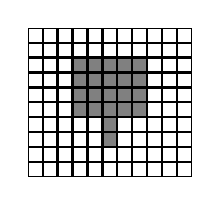
\begin{tikzpicture}
                \matrix (img) [se,minimum width=0.5em, minimum height=0.5em] {
                    \node[bg] {}; \& \node[bg] {}; \& \node[bg] {}; \& \node[bg] {}; \&	\node[bg] {}; \& \node[bg] {}; \& \node[bg] {}; \& \node[bg] {}; \&	\node[bg] {}; \& \node[bg] {}; \& \node[bg] {}; \\
                    \node[bg] {}; \& \node[bg] {}; \& \node[bg] {}; \& \node[bg] {}; \&	\node[bg] {}; \& \node[bg] {}; \& \node[bg] {}; \& \node[bg] {}; \&	\node[bg] {}; \& \node[bg] {}; \& \node[bg] {}; \\
                    \node[bg] {}; \& \node[bg] {}; \& \node[bg] {}; \& \node[fg] {}; \&	\node[fg] {}; \& \node[fg] {}; \& \node[fg] {}; \& \node[fg] {}; \&	\node[bg] {}; \& \node[bg] {}; \& \node[bg] {}; \\
                    \node[bg] {}; \& \node[bg] {}; \& \node[bg] {}; \& \node[fg] {}; \&	\node[fg] {}; \& \node[fg] {}; \& \node[fg] {}; \& \node[fg] {}; \&	\node[bg] {}; \& \node[bg] {}; \& \node[bg] {}; \\
                    \node[bg] {}; \& \node[bg] {}; \& \node[bg] {}; \& \node[fg] {}; \&	\node[fg] {}; \& \node[fg] {}; \& \node[fg] {}; \& \node[fg] {}; \&	\node[bg] {}; \& \node[bg] {}; \& \node[bg] {}; \\
                    \node[bg] {}; \& \node[bg] {}; \& \node[bg] {}; \& \node[fg] {}; \&	\node[fg] {}; \& \node[fg] {}; \& \node[fg] {}; \& \node[fg] {}; \&	\node[bg] {}; \& \node[bg] {}; \& \node[bg] {}; \\
                    \node[bg] {}; \& \node[bg] {}; \& \node[bg] {}; \& \node[bg] {}; \&	\node[bg] {}; \& \node[fg] {}; \& \node[bg] {}; \& \node[bg] {}; \&	\node[bg] {}; \& \node[bg] {}; \& \node[bg] {}; \\
                    \node[bg] {}; \& \node[bg] {}; \& \node[bg] {}; \& \node[bg] {}; \&	\node[bg] {}; \& \node[fg] {}; \& \node[bg] {}; \& \node[bg] {}; \&	\node[bg] {}; \& \node[bg] {}; \& \node[bg] {}; \\
                    \node[bg] {}; \& \node[bg] {}; \& \node[bg] {}; \& \node[bg] {}; \&	\node[bg] {}; \& \node[bg] {}; \& \node[bg] {}; \& \node[bg] {}; \&	\node[bg] {}; \& \node[bg] {}; \& \node[bg] {}; \\
                    \node[bg] {}; \& \node[bg] {}; \& \node[bg] {}; \& \node[bg] {}; \&	\node[bg] {}; \& \node[bg] {}; \& \node[bg] {}; \& \node[bg] {}; \&	\node[bg] {}; \& \node[bg] {}; \& \node[bg] {}; \\
                };
            \end{tikzpicture}
        }
        $\rightarrow$
        \raisebox{-0.07\textwidth}{
            \tikzsetnextfilename{openinginput}
            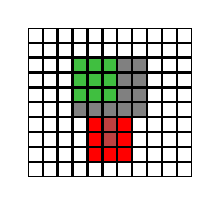
\begin{tikzpicture}
                \matrix (img) [se,minimum width=0.5em, minimum height=0.5em] {
                    \node[bg] {}; \& \node[bg] {}; \& \node[bg] {}; \& \node[bg] {}; \&	\node[bg] {}; \& \node[bg] {}; \& \node[bg] {}; \& \node[bg] {}; \&	\node[bg] {}; \& \node[bg] {}; \& \node[bg] {}; \\
                    \node[bg] {}; \& \node[bg] {}; \& \node[bg] {}; \& \node[bg] {}; \&	\node[bg] {}; \& \node[bg] {}; \& \node[bg] {}; \& \node[bg] {}; \&	\node[bg] {}; \& \node[bg] {}; \& \node[bg] {}; \\
                    \node[bg] {}; \& \node[bg] {}; \& \node[bg] {}; \& \node[sepm] {}; \&	\node[sepm] {}; \& \node[sepm] {}; \& \node[fg] {}; \& \node[fg] {}; \&	\node[bg] {}; \& \node[bg] {}; \& \node[bg] {}; \\
                    \node[bg] {}; \& \node[bg] {}; \& \node[bg] {}; \& \node[sepm] {}; \&	\node[sepm] {}; \& \node[sepm] {}; \& \node[fg] {}; \& \node[fg] {}; \&	\node[bg] {}; \& \node[bg] {}; \& \node[bg] {}; \\
                    \node[bg] {}; \& \node[bg] {}; \& \node[bg] {}; \& \node[sepm] {}; \&	\node[sepm] {}; \& \node[sepm] {}; \& \node[fg] {}; \& \node[fg] {}; \&	\node[bg] {}; \& \node[bg] {}; \& \node[bg] {}; \\
                    \node[bg] {}; \& \node[bg] {}; \& \node[bg] {}; \& \node[fg] {}; \&	\node[fg] {}; \& \node[fg] {}; \& \node[fg] {}; \& \node[fg] {}; \&	\node[bg] {}; \& \node[bg] {}; \& \node[bg] {}; \\
                    \node[bg] {}; \& \node[bg] {}; \& \node[bg] {}; \& \node[bg] {}; \&	\node[sen] {}; \& \node[senm] {}; \& \node[sen] {}; \& \node[bg] {}; \&	\node[bg] {}; \& \node[bg] {}; \& \node[bg] {}; \\
                    \node[bg] {}; \& \node[bg] {}; \& \node[bg] {}; \& \node[bg] {}; \&	\node[sen] {}; \& \node[senm] {}; \& \node[sen] {}; \& \node[bg] {}; \&	\node[bg] {}; \& \node[bg] {}; \& \node[bg] {}; \\
                    \node[bg] {}; \& \node[bg] {}; \& \node[bg] {}; \& \node[bg] {}; \&	\node[sen] {}; \& \node[sen] {}; \& \node[sen] {}; \& \node[bg] {}; \&	\node[bg] {}; \& \node[bg] {}; \& \node[bg] {}; \\
                    \node[bg] {}; \& \node[bg] {}; \& \node[bg] {}; \& \node[bg] {}; \&	\node[bg] {}; \& \node[bg] {}; \& \node[bg] {}; \& \node[bg] {}; \&	\node[bg] {}; \& \node[bg] {}; \& \node[bg] {}; \\
                };
            \end{tikzpicture}
        }
        $\rightarrow$
        \raisebox{-0.07\textwidth}{
            \tikzsetnextfilename{resultopening1}
            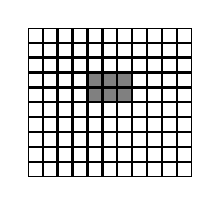
\begin{tikzpicture}
                \matrix (img) [se,minimum width=0.5em, minimum height=0.5em] {
                    \node[bg] {}; \& \node[bg] {}; \& \node[bg] {}; \& \node[bg] {}; \&	\node[bg] {}; \& \node[bg] {}; \& \node[bg] {}; \& \node[bg] {}; \&	\node[bg] {}; \& \node[bg] {}; \& \node[bg] {}; \\
                    \node[bg] {}; \& \node[bg] {}; \& \node[bg] {}; \& \node[bg] {}; \&	\node[bg] {}; \& \node[bg] {}; \& \node[bg] {}; \& \node[bg] {}; \&	\node[bg] {}; \& \node[bg] {}; \& \node[bg] {}; \\
                    \node[bg] {}; \& \node[bg] {}; \& \node[bg] {}; \& \node[bg] {}; \&	\node[bg] {}; \& \node[bg] {}; \& \node[bg] {}; \& \node[bg] {}; \&	\node[bg] {}; \& \node[bg] {}; \& \node[bg] {}; \\
                    \node[bg] {}; \& \node[bg] {}; \& \node[bg] {}; \& \node[bg] {}; \&	\node[fg] {}; \& \node[fg] {}; \& \node[fg] {}; \& \node[bg] {}; \&	\node[bg] {}; \& \node[bg] {}; \& \node[bg] {}; \\
                    \node[bg] {}; \& \node[bg] {}; \& \node[bg] {}; \& \node[bg] {}; \&	\node[fg] {}; \& \node[fg] {}; \& \node[fg] {}; \& \node[bg] {}; \&	\node[bg] {}; \& \node[bg] {}; \& \node[bg] {}; \\
                    \node[bg] {}; \& \node[bg] {}; \& \node[bg] {}; \& \node[bg] {}; \&	\node[bg] {}; \& \node[bg] {}; \& \node[bg] {}; \& \node[bg] {}; \&	\node[bg] {}; \& \node[bg] {}; \& \node[bg] {}; \\
                    \node[bg] {}; \& \node[bg] {}; \& \node[bg] {}; \& \node[bg] {}; \&	\node[bg] {}; \& \node[bg] {}; \& \node[bg] {}; \& \node[bg] {}; \&	\node[bg] {}; \& \node[bg] {}; \& \node[bg] {}; \\
                    \node[bg] {}; \& \node[bg] {}; \& \node[bg] {}; \& \node[bg] {}; \&	\node[bg] {}; \& \node[bg] {}; \& \node[bg] {}; \& \node[bg] {}; \&	\node[bg] {}; \& \node[bg] {}; \& \node[bg] {}; \\
                    \node[bg] {}; \& \node[bg] {}; \& \node[bg] {}; \& \node[bg] {}; \&	\node[bg] {}; \& \node[bg] {}; \& \node[bg] {}; \& \node[bg] {}; \&	\node[bg] {}; \& \node[bg] {}; \& \node[bg] {}; \\
                    \node[bg] {}; \& \node[bg] {}; \& \node[bg] {}; \& \node[bg] {}; \&	\node[bg] {}; \& \node[bg] {}; \& \node[bg] {}; \& \node[bg] {}; \&	\node[bg] {}; \& \node[bg] {}; \& \node[bg] {}; \\
                };
            \end{tikzpicture}
        }
        \\[0.8em]
        Dilation\\[0.1em]
        \raisebox{-0.07\textwidth}{
            \tikzsetnextfilename{resultopening1}
            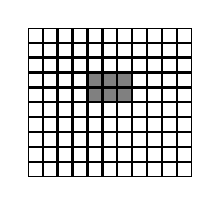
\begin{tikzpicture}
                \matrix (img) [se,minimum width=0.5em, minimum height=0.5em] {
                    \node[bg] {}; \& \node[bg] {}; \& \node[bg] {}; \& \node[bg] {}; \&	\node[bg] {}; \& \node[bg] {}; \& \node[bg] {}; \& \node[bg] {}; \&	\node[bg] {}; \& \node[bg] {}; \& \node[bg] {}; \\
                    \node[bg] {}; \& \node[bg] {}; \& \node[bg] {}; \& \node[bg] {}; \&	\node[bg] {}; \& \node[bg] {}; \& \node[bg] {}; \& \node[bg] {}; \&	\node[bg] {}; \& \node[bg] {}; \& \node[bg] {}; \\
                    \node[bg] {}; \& \node[bg] {}; \& \node[bg] {}; \& \node[bg] {}; \&	\node[bg] {}; \& \node[bg] {}; \& \node[bg] {}; \& \node[bg] {}; \&	\node[bg] {}; \& \node[bg] {}; \& \node[bg] {}; \\
                    \node[bg] {}; \& \node[bg] {}; \& \node[bg] {}; \& \node[bg] {}; \&	\node[fg] {}; \& \node[fg] {}; \& \node[fg] {}; \& \node[bg] {}; \&	\node[bg] {}; \& \node[bg] {}; \& \node[bg] {}; \\
                    \node[bg] {}; \& \node[bg] {}; \& \node[bg] {}; \& \node[bg] {}; \&	\node[fg] {}; \& \node[fg] {}; \& \node[fg] {}; \& \node[bg] {}; \&	\node[bg] {}; \& \node[bg] {}; \& \node[bg] {}; \\
                    \node[bg] {}; \& \node[bg] {}; \& \node[bg] {}; \& \node[bg] {}; \&	\node[bg] {}; \& \node[bg] {}; \& \node[bg] {}; \& \node[bg] {}; \&	\node[bg] {}; \& \node[bg] {}; \& \node[bg] {}; \\
                    \node[bg] {}; \& \node[bg] {}; \& \node[bg] {}; \& \node[bg] {}; \&	\node[bg] {}; \& \node[bg] {}; \& \node[bg] {}; \& \node[bg] {}; \&	\node[bg] {}; \& \node[bg] {}; \& \node[bg] {}; \\
                    \node[bg] {}; \& \node[bg] {}; \& \node[bg] {}; \& \node[bg] {}; \&	\node[bg] {}; \& \node[bg] {}; \& \node[bg] {}; \& \node[bg] {}; \&	\node[bg] {}; \& \node[bg] {}; \& \node[bg] {}; \\
                    \node[bg] {}; \& \node[bg] {}; \& \node[bg] {}; \& \node[bg] {}; \&	\node[bg] {}; \& \node[bg] {}; \& \node[bg] {}; \& \node[bg] {}; \&	\node[bg] {}; \& \node[bg] {}; \& \node[bg] {}; \\
                    \node[bg] {}; \& \node[bg] {}; \& \node[bg] {}; \& \node[bg] {}; \&	\node[bg] {}; \& \node[bg] {}; \& \node[bg] {}; \& \node[bg] {}; \&	\node[bg] {}; \& \node[bg] {}; \& \node[bg] {}; \\
                };
            \end{tikzpicture}
        }
        $\rightarrow$
        \raisebox{-0.07\textwidth}{
            \tikzsetnextfilename{opening1}
            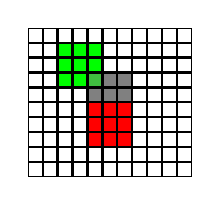
\begin{tikzpicture}
                \matrix (img) [se,minimum width=0.5em, minimum height=0.5em] {
                    \node[bg] {}; \& \node[bg] {}; \& \node[bg] {}; \& \node[bg] {}; \&	\node[bg] {}; \& \node[bg] {}; \& \node[bg] {}; \& \node[bg] {}; \&	\node[bg] {}; \& \node[bg] {}; \& \node[bg] {}; \\
                    \node[bg] {}; \& \node[bg] {}; \& \node[sep] {}; \& \node[sep] {}; \&	\node[sep] {}; \& \node[bg] {}; \& \node[bg] {}; \& \node[bg] {}; \&	\node[bg] {}; \& \node[bg] {}; \& \node[bg] {}; \\
                    \node[bg] {}; \& \node[bg] {}; \& \node[sep] {}; \& \node[sep] {}; \&	\node[sep] {}; \& \node[bg] {}; \& \node[bg] {}; \& \node[bg] {}; \&	\node[bg] {}; \& \node[bg] {}; \& \node[bg] {}; \\
                    \node[bg] {}; \& \node[bg] {}; \& \node[sep] {}; \& \node[sep] {}; \&	\node[sepm] {}; \& \node[fg] {}; \& \node[fg] {}; \& \node[bg] {}; \&	\node[bg] {}; \& \node[bg] {}; \& \node[bg] {}; \\
                    \node[bg] {}; \& \node[bg] {}; \& \node[bg] {}; \& \node[bg] {}; \&	\node[fg] {}; \& \node[fg] {}; \& \node[fg] {}; \& \node[bg] {}; \&	\node[bg] {}; \& \node[bg] {}; \& \node[bg] {}; \\
                    \node[bg] {}; \& \node[bg] {}; \& \node[bg] {}; \& \node[bg] {}; \&	\node[sen] {}; \& \node[sen] {}; \& \node[sen] {}; \& \node[bg] {}; \&	\node[bg] {}; \& \node[bg] {}; \& \node[bg] {}; \\
                    \node[bg] {}; \& \node[bg] {}; \& \node[bg] {}; \& \node[bg] {}; \&	\node[sen] {}; \& \node[sen] {}; \& \node[sen] {}; \& \node[bg] {}; \&	\node[bg] {}; \& \node[bg] {}; \& \node[bg] {}; \\
                    \node[bg] {}; \& \node[bg] {}; \& \node[bg] {}; \& \node[bg] {}; \&	\node[sen] {}; \& \node[sen] {}; \& \node[sen] {}; \& \node[bg] {}; \&	\node[bg] {}; \& \node[bg] {}; \& \node[bg] {}; \\
                    \node[bg] {}; \& \node[bg] {}; \& \node[bg] {}; \& \node[bg] {}; \&	\node[bg] {}; \& \node[bg] {}; \& \node[bg] {}; \& \node[bg] {}; \&	\node[bg] {}; \& \node[bg] {}; \& \node[bg] {}; \\
                    \node[bg] {}; \& \node[bg] {}; \& \node[bg] {}; \& \node[bg] {}; \&	\node[bg] {}; \& \node[bg] {}; \& \node[bg] {}; \& \node[bg] {}; \&	\node[bg] {}; \& \node[bg] {}; \& \node[bg] {}; \\
                };
            \end{tikzpicture}
        }
        $\rightarrow$
        \raisebox{-0.07\textwidth}{
            \tikzsetnextfilename{opening2}
            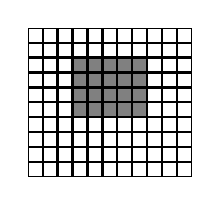
\begin{tikzpicture}
                \matrix (img) [se,minimum width=0.5em, minimum height=0.5em] {
                    \node[bg] {}; \& \node[bg] {}; \& \node[bg] {}; \& \node[bg] {}; \&	\node[bg] {}; \& \node[bg] {}; \& \node[bg] {}; \& \node[bg] {}; \&	\node[bg] {}; \& \node[bg] {}; \& \node[bg] {}; \\
                    \node[bg] {}; \& \node[bg] {}; \& \node[bg] {}; \& \node[bg] {}; \&	\node[bg] {}; \& \node[bg] {}; \& \node[bg] {}; \& \node[bg] {}; \&	\node[bg] {}; \& \node[bg] {}; \& \node[bg] {}; \\
                    \node[bg] {}; \& \node[bg] {}; \& \node[bg] {}; \& \node[fg] {}; \&	\node[fg] {}; \& \node[fg] {}; \& \node[fg] {}; \& \node[fg] {}; \&	\node[bg] {}; \& \node[bg] {}; \& \node[bg] {}; \\
                    \node[bg] {}; \& \node[bg] {}; \& \node[bg] {}; \& \node[fg] {}; \&	\node[fg] {}; \& \node[fg] {}; \& \node[fg] {}; \& \node[fg] {}; \&	\node[bg] {}; \& \node[bg] {}; \& \node[bg] {}; \\
                    \node[bg] {}; \& \node[bg] {}; \& \node[bg] {}; \& \node[fg] {}; \&	\node[fg] {}; \& \node[fg] {}; \& \node[fg] {}; \& \node[fg] {}; \&	\node[bg] {}; \& \node[bg] {}; \& \node[bg] {}; \\
                    \node[bg] {}; \& \node[bg] {}; \& \node[bg] {}; \& \node[fg] {}; \&	\node[fg] {}; \& \node[fg] {}; \& \node[fg] {}; \& \node[fg] {}; \&	\node[bg] {}; \& \node[bg] {}; \& \node[bg] {}; \\
                    \node[bg] {}; \& \node[bg] {}; \& \node[bg] {}; \& \node[bg] {}; \&	\node[bg] {}; \& \node[bg] {}; \& \node[bg] {}; \& \node[bg] {}; \&	\node[bg] {}; \& \node[bg] {}; \& \node[bg] {}; \\
                    \node[bg] {}; \& \node[bg] {}; \& \node[bg] {}; \& \node[bg] {}; \&	\node[bg] {}; \& \node[bg] {}; \& \node[bg] {}; \& \node[bg] {}; \&	\node[bg] {}; \& \node[bg] {}; \& \node[bg] {}; \\
                    \node[bg] {}; \& \node[bg] {}; \& \node[bg] {}; \& \node[bg] {}; \&	\node[bg] {}; \& \node[bg] {}; \& \node[bg] {}; \& \node[bg] {}; \&	\node[bg] {}; \& \node[bg] {}; \& \node[bg] {}; \\
                    \node[bg] {}; \& \node[bg] {}; \& \node[bg] {}; \& \node[bg] {}; \&	\node[bg] {}; \& \node[bg] {}; \& \node[bg] {}; \& \node[bg] {}; \&	\node[bg] {}; \& \node[bg] {}; \& \node[bg] {}; \\
                };
            \end{tikzpicture}
        }
    \end{center}
\end{frame}

\begin{frame}
    \frametitle{Morphological Operations}
    \begin{block}{Closing}
        $\mathrm{F} \bullet \mathrm{S} = (\mathrm{F}\oplus \mathrm{S})\ominus \mathrm{S}$
    \end{block}
    \begin{center}
        Dilation\\[0.1em]
        \raisebox{-0.07\textwidth}{
            \tikzsetnextfilename{erosioninput}
            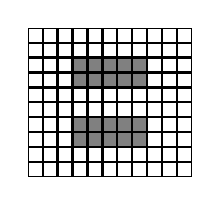
\begin{tikzpicture}
                \matrix (img) [se,minimum width=0.5em, minimum height=0.5em] {
                    \node[bg] {}; \& \node[bg] {}; \& \node[bg] {}; \& \node[bg] {}; \&	\node[bg] {}; \& \node[bg] {}; \& \node[bg] {}; \& \node[bg] {}; \&	\node[bg] {}; \& \node[bg] {}; \& \node[bg] {}; \\
                    \node[bg] {}; \& \node[bg] {}; \& \node[bg] {}; \& \node[bg] {}; \&	\node[bg] {}; \& \node[bg] {}; \& \node[bg] {}; \& \node[bg] {}; \&	\node[bg] {}; \& \node[bg] {}; \& \node[bg] {}; \\
                    \node[bg] {}; \& \node[bg] {}; \& \node[bg] {}; \& \node[fg] {}; \&	\node[fg] {}; \& \node[fg] {}; \& \node[fg] {}; \& \node[fg] {}; \&	\node[bg] {}; \& \node[bg] {}; \& \node[bg] {}; \\
                    \node[bg] {}; \& \node[bg] {}; \& \node[bg] {}; \& \node[fg] {}; \&	\node[fg] {}; \& \node[fg] {}; \& \node[fg] {}; \& \node[fg] {}; \&	\node[bg] {}; \& \node[bg] {}; \& \node[bg] {}; \\
                    \node[bg] {}; \& \node[bg] {}; \& \node[bg] {}; \& \node[bg] {}; \&	\node[bg] {}; \& \node[bg] {}; \& \node[bg] {}; \& \node[bg] {}; \&	\node[bg] {}; \& \node[bg] {}; \& \node[bg] {}; \\
                    \node[bg] {}; \& \node[bg] {}; \& \node[bg] {}; \& \node[bg] {}; \&	\node[bg] {}; \& \node[bg] {}; \& \node[bg] {}; \& \node[bg] {}; \&	\node[bg] {}; \& \node[bg] {}; \& \node[bg] {}; \\
                    \node[bg] {}; \& \node[bg] {}; \& \node[bg] {}; \& \node[fg] {}; \&	\node[fg] {}; \& \node[fg] {}; \& \node[fg] {}; \& \node[fg] {}; \&	\node[bg] {}; \& \node[bg] {}; \& \node[bg] {}; \\
                    \node[bg] {}; \& \node[bg] {}; \& \node[bg] {}; \& \node[fg] {}; \&	\node[fg] {}; \& \node[fg] {}; \& \node[fg] {}; \& \node[fg] {}; \&	\node[bg] {}; \& \node[bg] {}; \& \node[bg] {}; \\
                    \node[bg] {}; \& \node[bg] {}; \& \node[bg] {}; \& \node[bg] {}; \&	\node[bg] {}; \& \node[bg] {}; \& \node[bg] {}; \& \node[bg] {}; \&	\node[bg] {}; \& \node[bg] {}; \& \node[bg] {}; \\
                    \node[bg] {}; \& \node[bg] {}; \& \node[bg] {}; \& \node[bg] {}; \&	\node[bg] {}; \& \node[bg] {}; \& \node[bg] {}; \& \node[bg] {}; \&	\node[bg] {}; \& \node[bg] {}; \& \node[bg] {}; \\
                };
            \end{tikzpicture}
        }
        $\rightarrow$
        \raisebox{-0.07\textwidth}{
            \tikzsetnextfilename{dilation}
            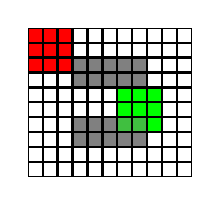
\begin{tikzpicture}
                \matrix (img) [se,minimum width=0.5em, minimum height=0.5em] {
                    \node[sen] {}; \& \node[sen] {}; \& \node[sen] {}; \& \node[bg] {}; \&	\node[bg] {}; \& \node[bg] {}; \& \node[bg] {}; \& \node[bg] {}; \&	\node[bg] {}; \& \node[bg] {}; \& \node[bg] {}; \\
                    \node[sen] {}; \& \node[sen] {}; \& \node[sen] {}; \& \node[bg] {}; \&	\node[bg] {}; \& \node[bg] {}; \& \node[bg] {}; \& \node[bg] {}; \&	\node[bg] {}; \& \node[bg] {}; \& \node[bg] {}; \\
                    \node[sen] {}; \& \node[sen] {}; \& \node[sen] {}; \& \node[fg] {}; \&	\node[fg] {}; \& \node[fg] {}; \& \node[fg] {}; \& \node[fg] {}; \&	\node[bg] {}; \& \node[bg] {}; \& \node[bg] {}; \\
                    \node[bg] {}; \& \node[bg] {}; \& \node[bg] {}; \& \node[fg] {}; \&	\node[fg] {}; \& \node[fg] {}; \& \node[fg] {}; \& \node[fg] {}; \&	\node[bg] {}; \& \node[bg] {}; \& \node[bg] {}; \\
                    \node[bg] {}; \& \node[bg] {}; \& \node[bg] {}; \& \node[bg] {}; \&	\node[bg] {}; \& \node[bg] {}; \& \node[sep] {}; \& \node[sep] {}; \&	\node[sep] {}; \& \node[bg] {}; \& \node[bg] {}; \\
                    \node[bg] {}; \& \node[bg] {}; \& \node[bg] {}; \& \node[bg] {}; \&	\node[bg] {}; \& \node[bg] {}; \& \node[sep] {}; \& \node[sep] {}; \&	\node[sep] {}; \& \node[bg] {}; \& \node[bg] {}; \\
                    \node[bg] {}; \& \node[bg] {}; \& \node[bg] {}; \& \node[fg] {}; \&	\node[fg] {}; \& \node[fg] {}; \& \node[sepm] {}; \& \node[sepm] {}; \&	\node[sep] {}; \& \node[bg] {}; \& \node[bg] {}; \\
                    \node[bg] {}; \& \node[bg] {}; \& \node[bg] {}; \& \node[fg] {}; \&	\node[fg] {}; \& \node[fg] {}; \& \node[fg] {}; \& \node[fg] {}; \&	\node[bg] {}; \& \node[bg] {}; \& \node[bg] {}; \\
                    \node[bg] {}; \& \node[bg] {}; \& \node[bg] {}; \& \node[bg] {}; \&	\node[bg] {}; \& \node[bg] {}; \& \node[bg] {}; \& \node[bg] {}; \&	\node[bg] {}; \& \node[bg] {}; \& \node[bg] {}; \\
                    \node[bg] {}; \& \node[bg] {}; \& \node[bg] {}; \& \node[bg] {}; \&	\node[bg] {}; \& \node[bg] {}; \& \node[bg] {}; \& \node[bg] {}; \&	\node[bg] {}; \& \node[bg] {}; \& \node[bg] {}; \\
                };
            \end{tikzpicture}
        }
        $\rightarrow$
        \raisebox{-0.07\textwidth}{
            \tikzsetnextfilename{dilationout}
            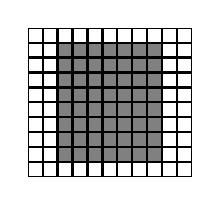
\begin{tikzpicture}
                \matrix (img) [se,minimum width=0.5em, minimum height=0.5em] {
                    \node[bg] {}; \& \node[bg] {}; \& \node[bg] {}; \& \node[bg] {}; \&	\node[bg] {}; \& \node[bg] {}; \& \node[bg] {}; \& \node[bg] {}; \&	\node[bg] {}; \& \node[bg] {}; \& \node[bg] {}; \\
                    \node[bg] {}; \& \node[bg] {}; \& \node[fg] {}; \& \node[fg] {}; \&	\node[fg] {}; \& \node[fg] {}; \& \node[fg] {}; \& \node[fg] {}; \&	\node[fg] {}; \& \node[bg] {}; \& \node[bg] {}; \\
                    \node[bg] {}; \& \node[bg] {}; \& \node[fg] {}; \& \node[fg] {}; \&	\node[fg] {}; \& \node[fg] {}; \& \node[fg] {}; \& \node[fg] {}; \&	\node[fg] {}; \& \node[bg] {}; \& \node[bg] {}; \\
                    \node[bg] {}; \& \node[bg] {}; \& \node[fg] {}; \& \node[fg] {}; \&	\node[fg] {}; \& \node[fg] {}; \& \node[fg] {}; \& \node[fg] {}; \&	\node[fg] {}; \& \node[bg] {}; \& \node[bg] {}; \\
                    \node[bg] {}; \& \node[bg] {}; \& \node[fg] {}; \& \node[fg] {}; \&	\node[fg] {}; \& \node[fg] {}; \& \node[fg] {}; \& \node[fg] {}; \&	\node[fg] {}; \& \node[bg] {}; \& \node[bg] {}; \\
                    \node[bg] {}; \& \node[bg] {}; \& \node[fg] {}; \& \node[fg] {}; \&	\node[fg] {}; \& \node[fg] {}; \& \node[fg] {}; \& \node[fg] {}; \&	\node[fg] {}; \& \node[bg] {}; \& \node[bg] {}; \\
                    \node[bg] {}; \& \node[bg] {}; \& \node[fg] {}; \& \node[fg] {}; \&	\node[fg] {}; \& \node[fg] {}; \& \node[fg] {}; \& \node[fg] {}; \&	\node[fg] {}; \& \node[bg] {}; \& \node[bg] {}; \\
                    \node[bg] {}; \& \node[bg] {}; \& \node[fg] {}; \& \node[fg] {}; \&	\node[fg] {}; \& \node[fg] {}; \& \node[fg] {}; \& \node[fg] {}; \&	\node[fg] {}; \& \node[bg] {}; \& \node[bg] {}; \\
                    \node[bg] {}; \& \node[bg] {}; \& \node[fg] {}; \& \node[fg] {}; \&	\node[fg] {}; \& \node[fg] {}; \& \node[fg] {}; \& \node[fg] {}; \&	\node[fg] {}; \& \node[bg] {}; \& \node[bg] {}; \\
                    \node[bg] {}; \& \node[bg] {}; \& \node[bg] {}; \& \node[bg] {}; \&	\node[bg] {}; \& \node[bg] {}; \& \node[bg] {}; \& \node[bg] {}; \&	\node[bg] {}; \& \node[bg] {}; \& \node[bg] {}; \\
                };
            \end{tikzpicture}
        }
        \\[0.8em]
        Erosion\\[0.1em]
        \raisebox{-0.07\textwidth}{
            \tikzsetnextfilename{erosionin}
            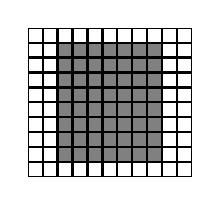
\begin{tikzpicture}
                \matrix (img) [se,minimum width=0.5em, minimum height=0.5em] {
                    \node[bg] {}; \& \node[bg] {}; \& \node[bg] {}; \& \node[bg] {}; \&	\node[bg] {}; \& \node[bg] {}; \& \node[bg] {}; \& \node[bg] {}; \&	\node[bg] {}; \& \node[bg] {}; \& \node[bg] {}; \\
                    \node[bg] {}; \& \node[bg] {}; \& \node[fg] {}; \& \node[fg] {}; \&	\node[fg] {}; \& \node[fg] {}; \& \node[fg] {}; \& \node[fg] {}; \&	\node[fg] {}; \& \node[bg] {}; \& \node[bg] {}; \\
                    \node[bg] {}; \& \node[bg] {}; \& \node[fg] {}; \& \node[fg] {}; \&	\node[fg] {}; \& \node[fg] {}; \& \node[fg] {}; \& \node[fg] {}; \&	\node[fg] {}; \& \node[bg] {}; \& \node[bg] {}; \\
                    \node[bg] {}; \& \node[bg] {}; \& \node[fg] {}; \& \node[fg] {}; \&	\node[fg] {}; \& \node[fg] {}; \& \node[fg] {}; \& \node[fg] {}; \&	\node[fg] {}; \& \node[bg] {}; \& \node[bg] {}; \\
                    \node[bg] {}; \& \node[bg] {}; \& \node[fg] {}; \& \node[fg] {}; \&	\node[fg] {}; \& \node[fg] {}; \& \node[fg] {}; \& \node[fg] {}; \&	\node[fg] {}; \& \node[bg] {}; \& \node[bg] {}; \\
                    \node[bg] {}; \& \node[bg] {}; \& \node[fg] {}; \& \node[fg] {}; \&	\node[fg] {}; \& \node[fg] {}; \& \node[fg] {}; \& \node[fg] {}; \&	\node[fg] {}; \& \node[bg] {}; \& \node[bg] {}; \\
                    \node[bg] {}; \& \node[bg] {}; \& \node[fg] {}; \& \node[fg] {}; \&	\node[fg] {}; \& \node[fg] {}; \& \node[fg] {}; \& \node[fg] {}; \&	\node[fg] {}; \& \node[bg] {}; \& \node[bg] {}; \\
                    \node[bg] {}; \& \node[bg] {}; \& \node[fg] {}; \& \node[fg] {}; \&	\node[fg] {}; \& \node[fg] {}; \& \node[fg] {}; \& \node[fg] {}; \&	\node[fg] {}; \& \node[bg] {}; \& \node[bg] {}; \\
                    \node[bg] {}; \& \node[bg] {}; \& \node[fg] {}; \& \node[fg] {}; \&	\node[fg] {}; \& \node[fg] {}; \& \node[fg] {}; \& \node[fg] {}; \&	\node[fg] {}; \& \node[bg] {}; \& \node[bg] {}; \\
                    \node[bg] {}; \& \node[bg] {}; \& \node[bg] {}; \& \node[bg] {}; \&	\node[bg] {}; \& \node[bg] {}; \& \node[bg] {}; \& \node[bg] {}; \&	\node[bg] {}; \& \node[bg] {}; \& \node[bg] {}; \\
                };
            \end{tikzpicture}
        }
        $\rightarrow$
        \raisebox{-0.07\textwidth}{
            \tikzsetnextfilename{erosion}
            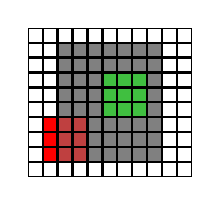
\begin{tikzpicture}
                \matrix (img) [se,minimum width=0.5em, minimum height=0.5em] {
                    \node[bg] {}; \& \node[bg] {}; \& \node[bg] {}; \& \node[bg] {}; \&	\node[bg] {}; \& \node[bg] {}; \& \node[bg] {}; \& \node[bg] {}; \&	\node[bg] {}; \& \node[bg] {}; \& \node[bg] {}; \\
                    \node[bg] {}; \& \node[bg] {}; \& \node[fg] {}; \& \node[fg] {}; \&	\node[fg] {}; \& \node[fg] {}; \& \node[fg] {}; \& \node[fg] {}; \&	\node[fg] {}; \& \node[bg] {}; \& \node[bg] {}; \\
                    \node[bg] {}; \& \node[bg] {}; \& \node[fg] {}; \& \node[fg] {}; \&	\node[fg] {}; \& \node[fg] {}; \& \node[fg] {}; \& \node[fg] {}; \&	\node[fg] {}; \& \node[bg] {}; \& \node[bg] {}; \\
                    \node[bg] {}; \& \node[bg] {}; \& \node[fg] {}; \& \node[fg] {}; \&	\node[fg] {}; \& \node[sepm] {}; \& \node[sepm] {}; \& \node[sepm] {}; \&	\node[fg] {}; \& \node[bg] {}; \& \node[bg] {}; \\
                    \node[bg] {}; \& \node[bg] {}; \& \node[fg] {}; \& \node[fg] {}; \&	\node[fg] {}; \& \node[sepm] {}; \& \node[sepm] {}; \& \node[sepm] {}; \&	\node[fg] {}; \& \node[bg] {}; \& \node[bg] {}; \\
                    \node[bg] {}; \& \node[bg] {}; \& \node[fg] {}; \& \node[fg] {}; \&	\node[fg] {}; \& \node[sepm] {}; \& \node[sepm] {}; \& \node[sepm] {}; \&	\node[fg] {}; \& \node[bg] {}; \& \node[bg] {}; \\
                    \node[bg] {}; \& \node[sen] {}; \& \node[senm] {}; \& \node[senm] {}; \&	\node[fg] {}; \& \node[fg] {}; \& \node[fg] {}; \& \node[fg] {}; \&	\node[fg] {}; \& \node[bg] {}; \& \node[bg] {}; \\
                    \node[bg] {}; \& \node[sen] {}; \& \node[senm] {}; \& \node[senm] {}; \&	\node[fg] {}; \& \node[fg] {}; \& \node[fg] {}; \& \node[fg] {}; \&	\node[fg] {}; \& \node[bg] {}; \& \node[bg] {}; \\
                    \node[bg] {}; \& \node[sen] {}; \& \node[senm] {}; \& \node[senm] {}; \&	\node[fg] {}; \& \node[fg] {}; \& \node[fg] {}; \& \node[fg] {}; \&	\node[fg] {}; \& \node[bg] {}; \& \node[bg] {}; \\
                    \node[bg] {}; \& \node[bg] {}; \& \node[bg] {}; \& \node[bg] {}; \&	\node[bg] {}; \& \node[bg] {}; \& \node[bg] {}; \& \node[bg] {}; \&	\node[bg] {}; \& \node[bg] {}; \& \node[bg] {}; \\
                };
            \end{tikzpicture}
        }
        $\rightarrow$
        \raisebox{-0.07\textwidth}{
            \tikzsetnextfilename{closingout}
            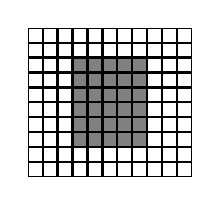
\begin{tikzpicture}
                \matrix (img) [se,minimum width=0.5em, minimum height=0.5em] {
                    \node[bg] {}; \& \node[bg] {}; \& \node[bg] {}; \& \node[bg] {}; \&	\node[bg] {}; \& \node[bg] {}; \& \node[bg] {}; \& \node[bg] {}; \&	\node[bg] {}; \& \node[bg] {}; \& \node[bg] {}; \\
                    \node[bg] {}; \& \node[bg] {}; \& \node[bg] {}; \& \node[bg] {}; \&	\node[bg] {}; \& \node[bg] {}; \& \node[bg] {}; \& \node[bg] {}; \&	\node[bg] {}; \& \node[bg] {}; \& \node[bg] {}; \\
                    \node[bg] {}; \& \node[bg] {}; \& \node[bg] {}; \& \node[fg] {}; \&	\node[fg] {}; \& \node[fg] {}; \& \node[fg] {}; \& \node[fg] {}; \&	\node[bg] {}; \& \node[bg] {}; \& \node[bg] {}; \\
                    \node[bg] {}; \& \node[bg] {}; \& \node[bg] {}; \& \node[fg] {}; \&	\node[fg] {}; \& \node[fg] {}; \& \node[fg] {}; \& \node[fg] {}; \&	\node[bg] {}; \& \node[bg] {}; \& \node[bg] {}; \\
                    \node[bg] {}; \& \node[bg] {}; \& \node[bg] {}; \& \node[fg] {}; \&	\node[fg] {}; \& \node[fg] {}; \& \node[fg] {}; \& \node[fg] {}; \&	\node[bg] {}; \& \node[bg] {}; \& \node[bg] {}; \\
                    \node[bg] {}; \& \node[bg] {}; \& \node[bg] {}; \& \node[fg] {}; \&	\node[fg] {}; \& \node[fg] {}; \& \node[fg] {}; \& \node[fg] {}; \&	\node[bg] {}; \& \node[bg] {}; \& \node[bg] {}; \\
                    \node[bg] {}; \& \node[bg] {}; \& \node[bg] {}; \& \node[fg] {}; \&	\node[fg] {}; \& \node[fg] {}; \& \node[fg] {}; \& \node[fg] {}; \&	\node[bg] {}; \& \node[bg] {}; \& \node[bg] {}; \\
                    \node[bg] {}; \& \node[bg] {}; \& \node[bg] {}; \& \node[fg] {}; \&	\node[fg] {}; \& \node[fg] {}; \& \node[fg] {}; \& \node[fg] {}; \&	\node[bg] {}; \& \node[bg] {}; \& \node[bg] {}; \\
                    \node[bg] {}; \& \node[bg] {}; \& \node[bg] {}; \& \node[bg] {}; \&	\node[bg] {}; \& \node[bg] {}; \& \node[bg] {}; \& \node[bg] {}; \&	\node[bg] {}; \& \node[bg] {}; \& \node[bg] {}; \\
                    \node[bg] {}; \& \node[bg] {}; \& \node[bg] {}; \& \node[bg] {}; \&	\node[bg] {}; \& \node[bg] {}; \& \node[bg] {}; \& \node[bg] {}; \&	\node[bg] {}; \& \node[bg] {}; \& \node[bg] {}; \\
                };
            \end{tikzpicture}
        }
    \end{center}
\end{frame}

%\begin{frame}
%  \frametitle{Correlation-based Motion Analysis}
%  \begin{block}{Normalized cross-correlation}
%    Images or ``region of interests'' (ROIs) $g_1,\,g_2$
%  \begin{equation*}
%    r(x',y')=\frac{\int\!\!\int g_1(x,y)\cdot
%      g_2(x+x',y+y')d\!xd\!y}{\sqrt{\int\!\!\int
%      g_1^2(x,y)d\!xd\!y\cdot\int\!\!\int g_2^2(x,y)d\!xd\!y}}
%  \end{equation*}
%  Motion $(\tilde{x},\tilde{y})$ between $g_1$ and $g_2$:
%  \begin{equation*}
%    \tilde{x},\tilde{y} = \arg\max_{x',y'}r(x',y')
%  \end{equation*}
%  \end{block}
%\end{frame}

\begin{frame}
    \frametitle{Deep Learning}
    \begin{center}
    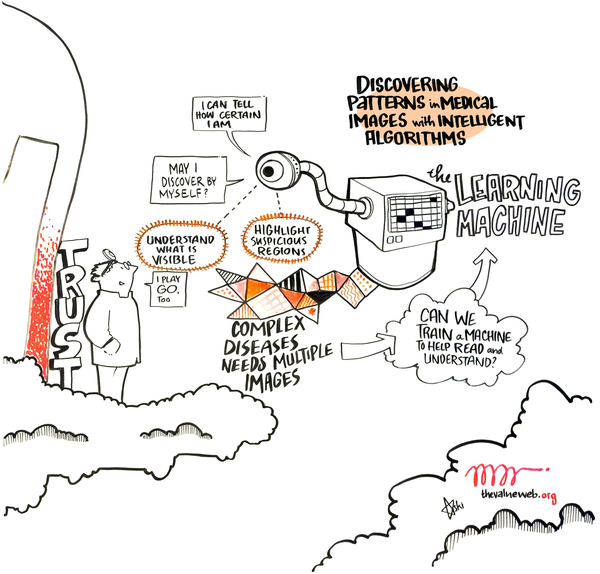
\includegraphics[height=6cm]{img/AI-Medical-600px.png}
    {\tiny Image credit Ben Glocker}
    \end{center}
\end{frame}

\begin{frame}
    \frametitle{Deep Learning}
    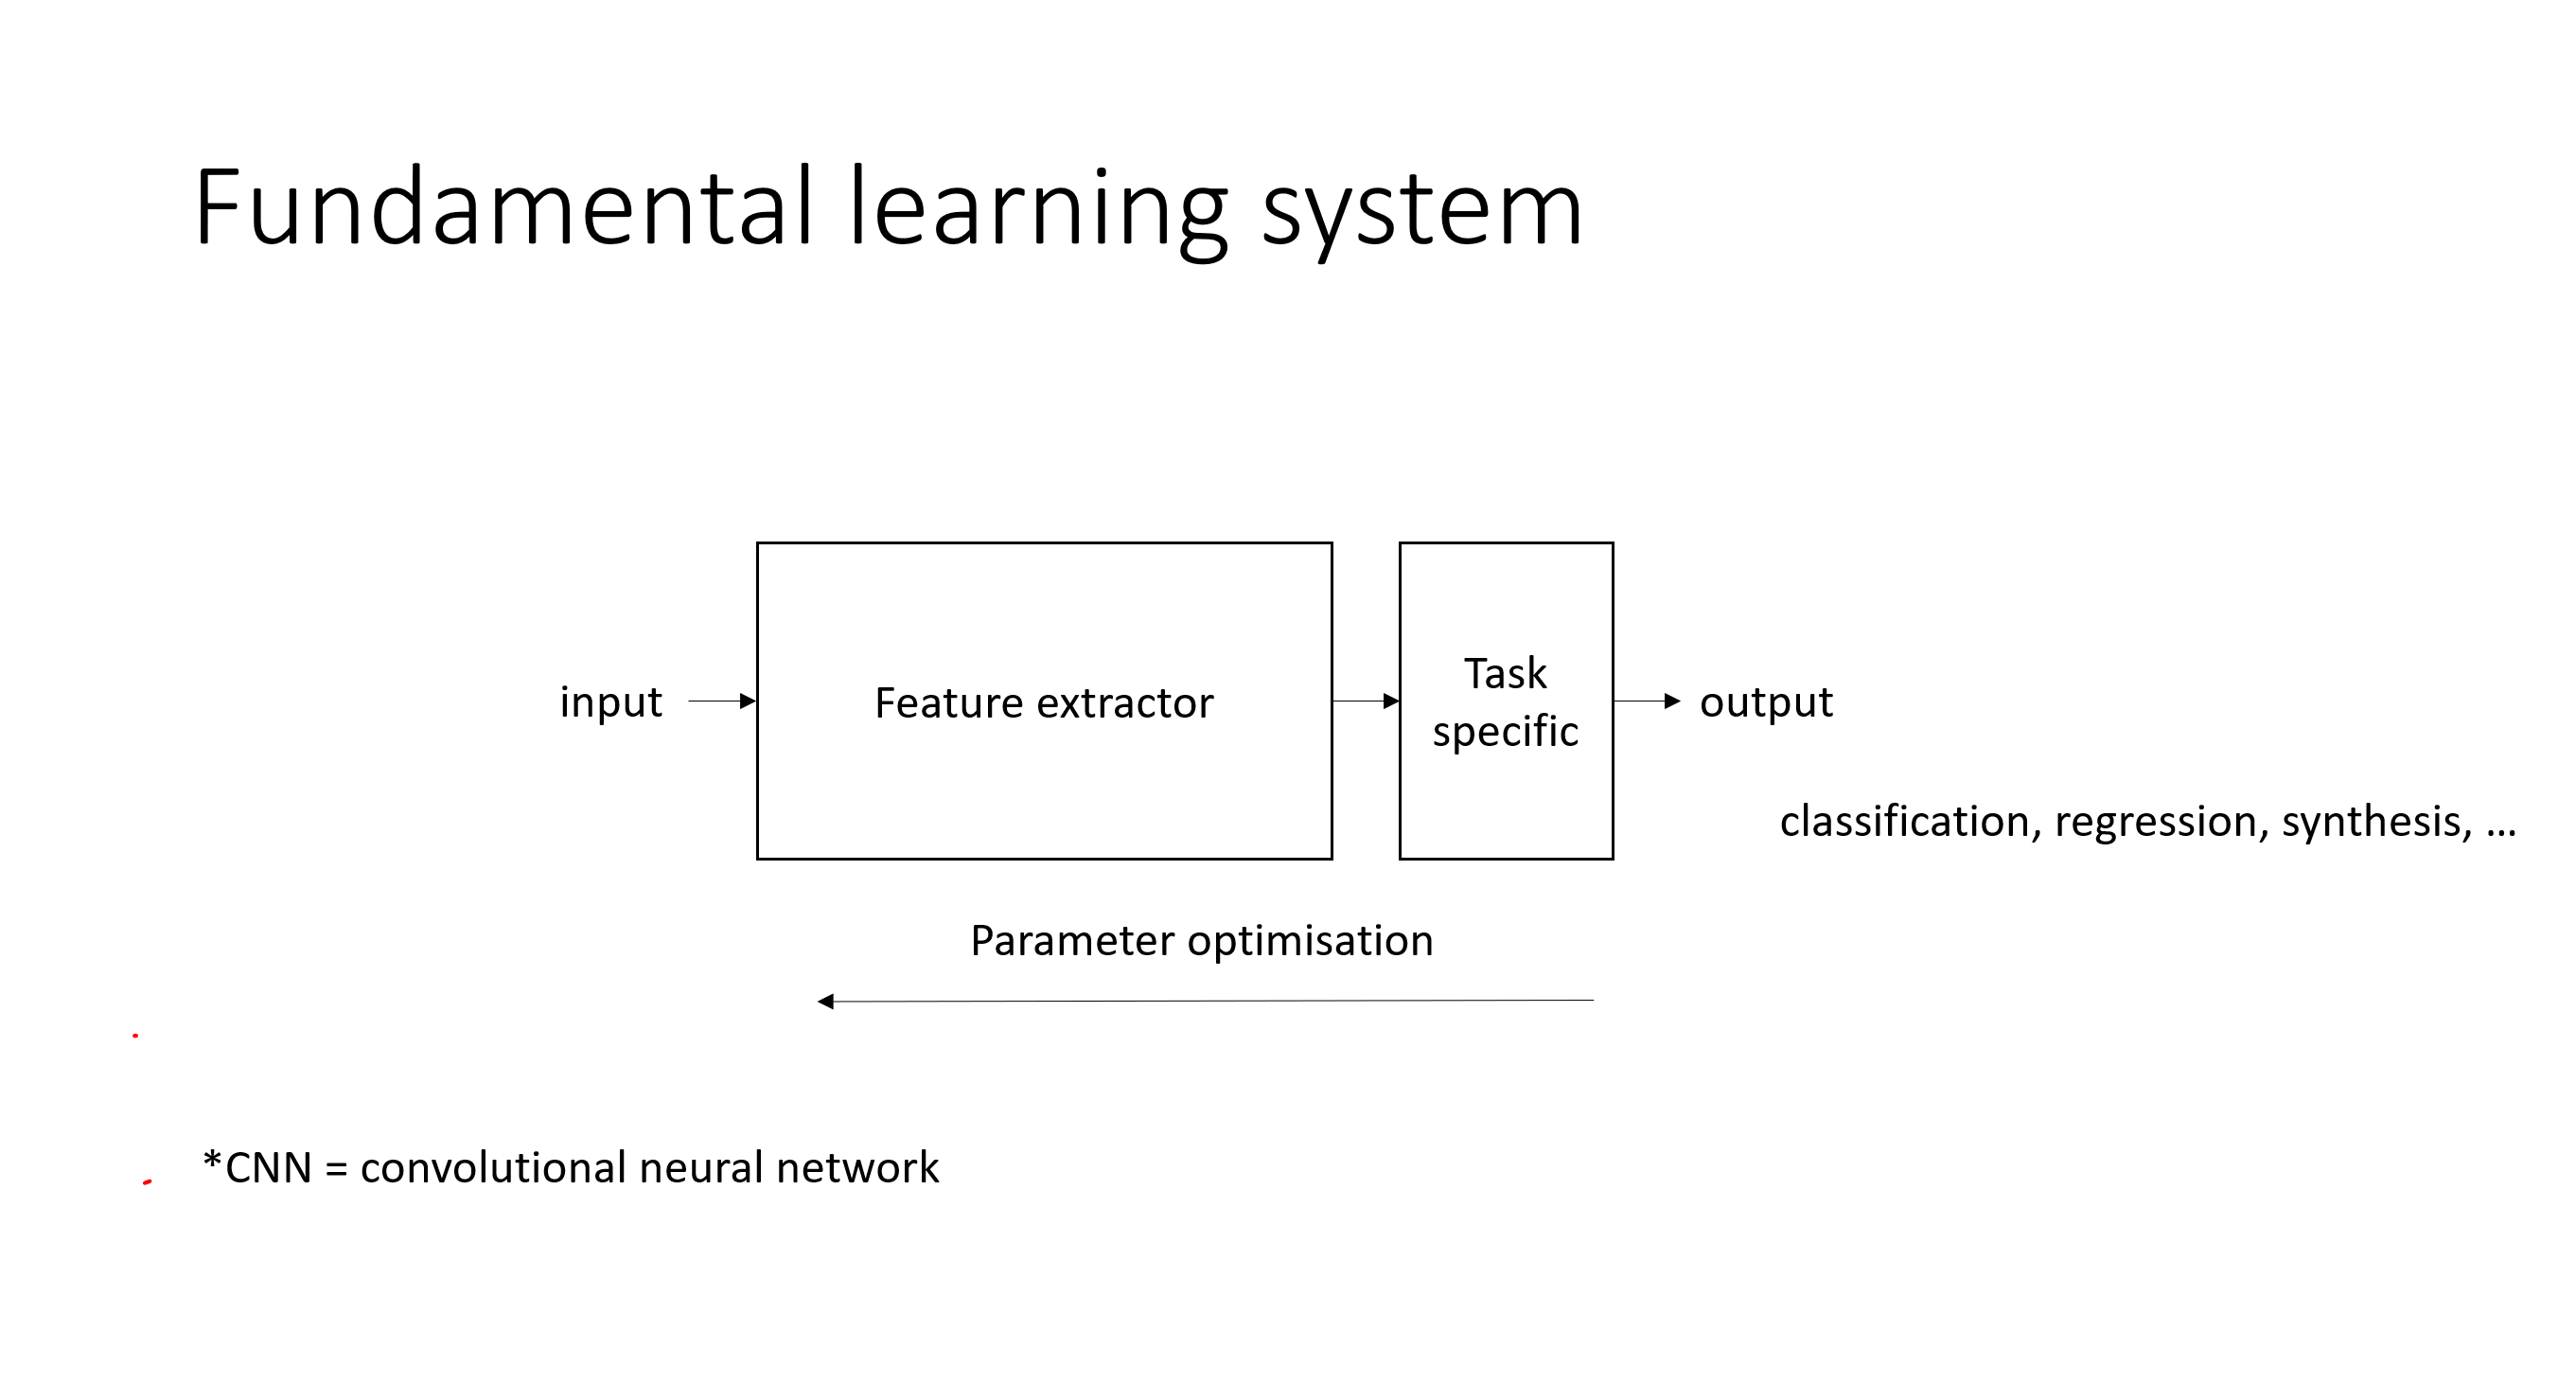
\includegraphics[height=6cm]{img/woCNN.png}
\end{frame}

\begin{frame}
    \frametitle{Deep Learning}
    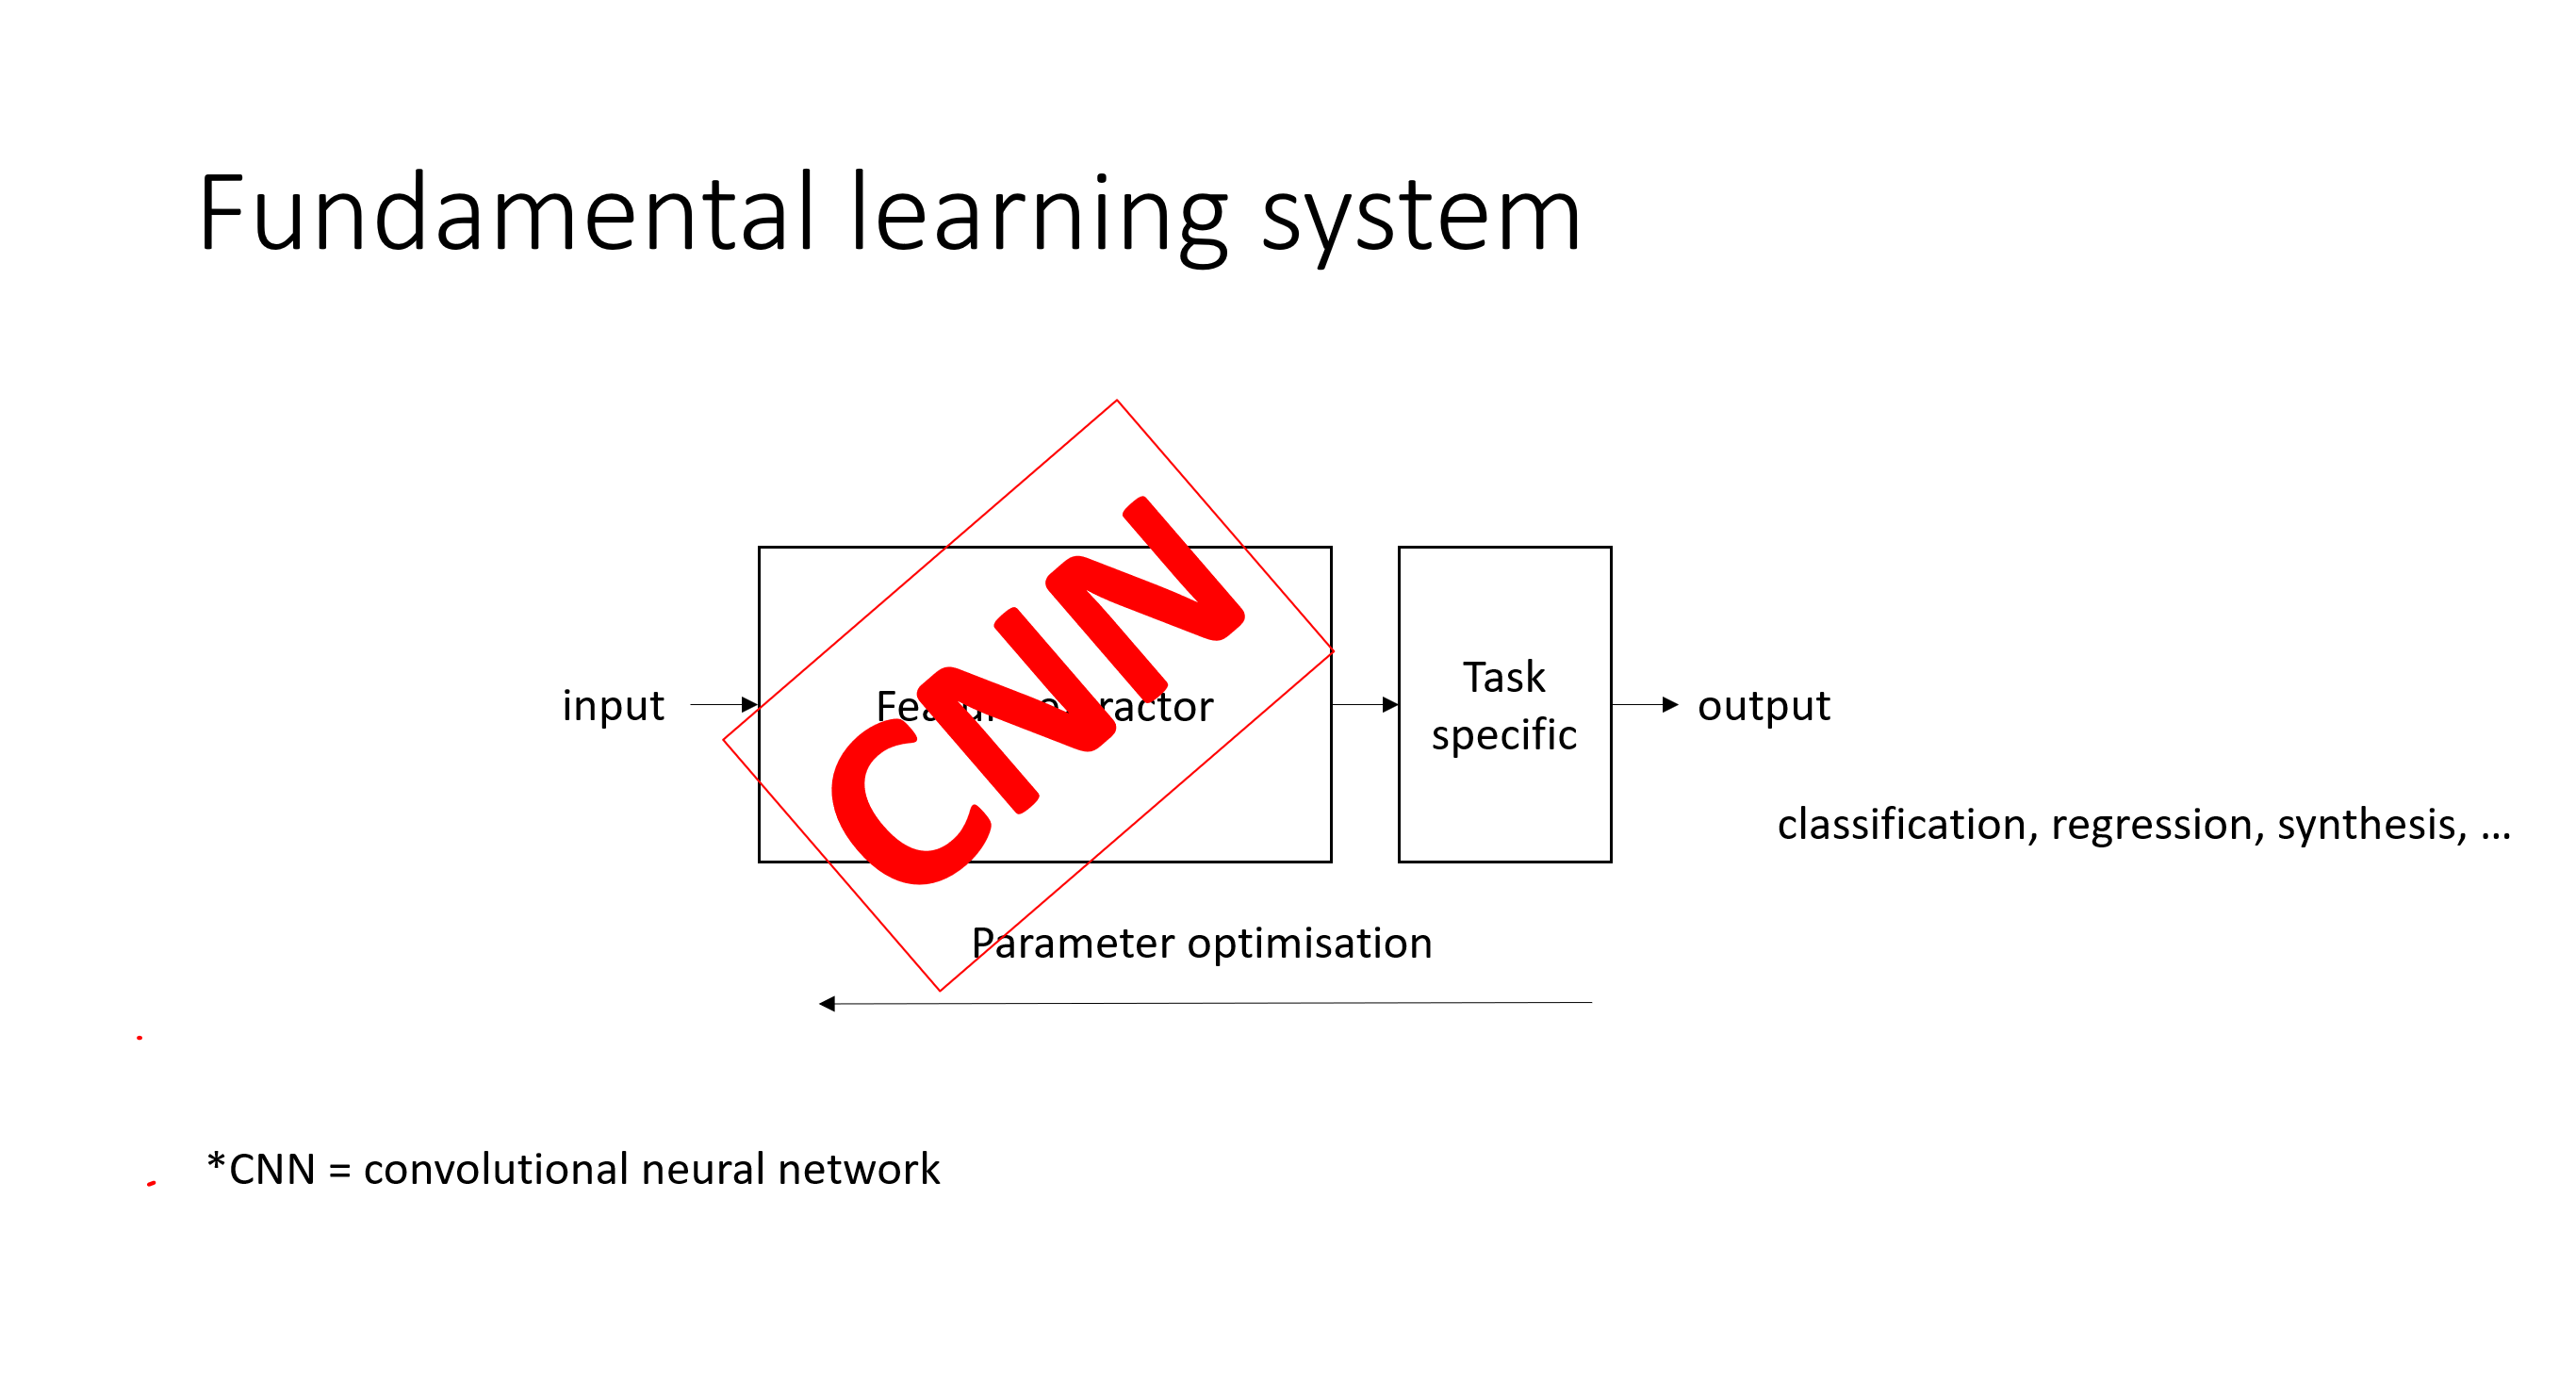
\includegraphics[height=6cm]{img/wCNN.png}
\end{frame}


\begin{frame}
    \frametitle{Deep Learning}
    \begin{itemize}
        \item generate a lot of samples (segmentations, calssification, etc.)
        \item use a learning framework (e.g. \url{https://github.com/MIC-DKFZ/nnUNet} for segmentation, Resnet for classification \url{https://pytorch.org/hub/pytorch_vision_resnet/})
        \item keep a certain split for validaiton and testing (e.g. 80:10:10), do cross-validation
        \item get good compute infrastructure (GPUs) train and test.
    \end{itemize}
    \begin{center}
 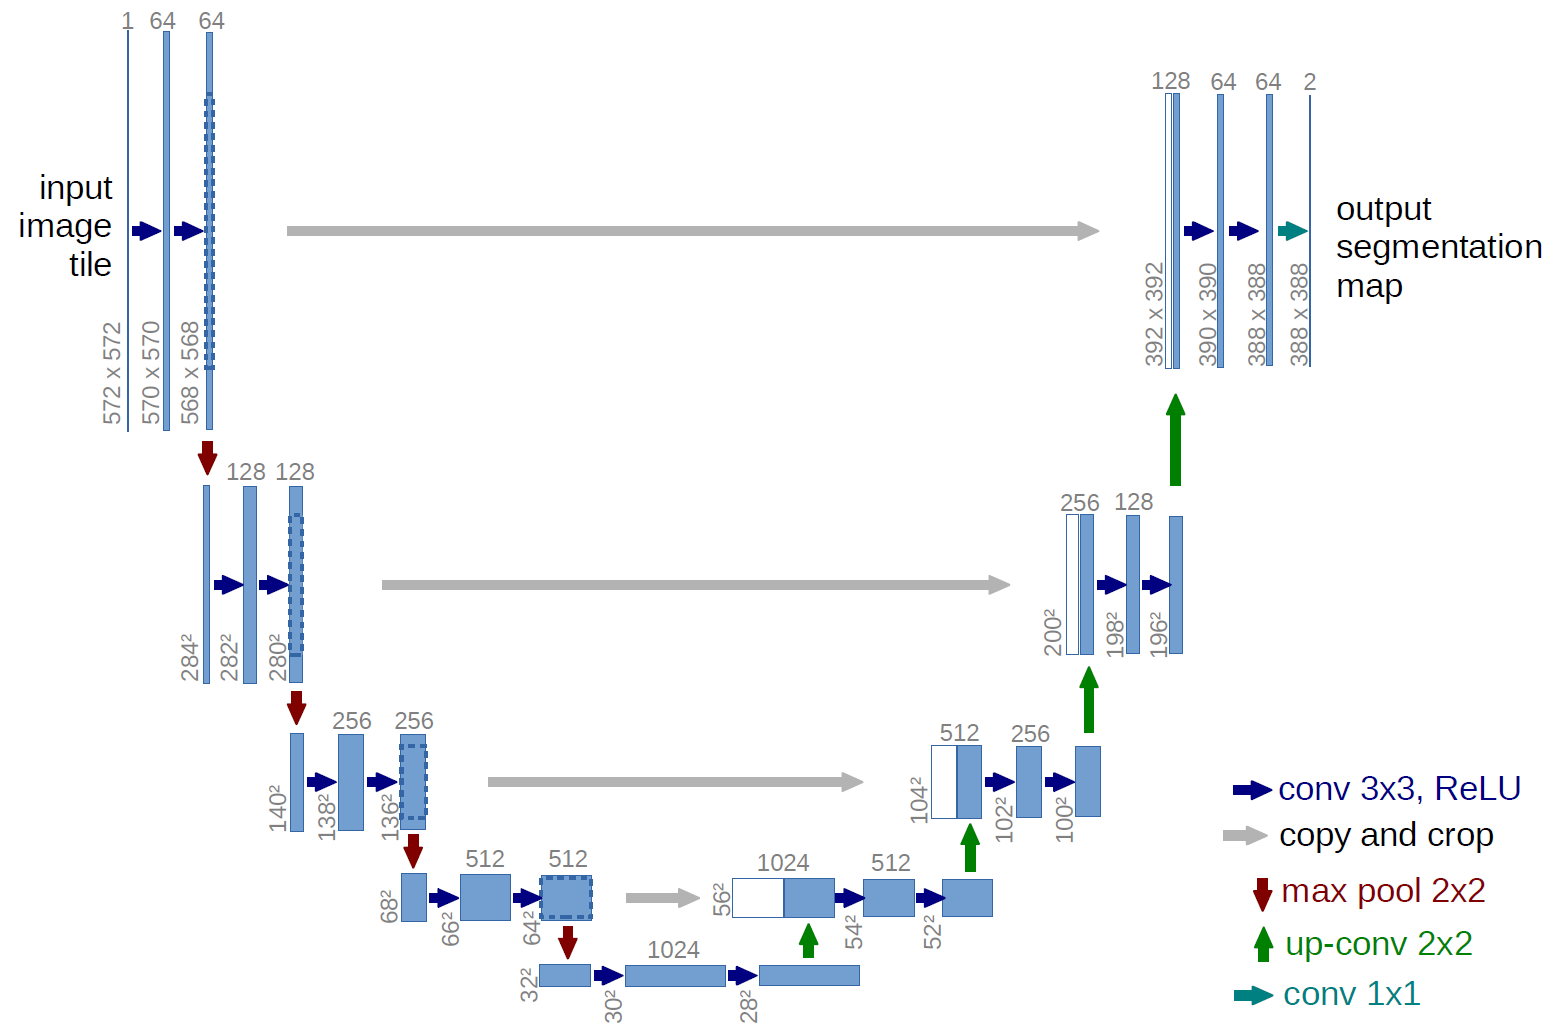
\includegraphics[height=4cm]{img/u-net-architecture.png}
{\tiny Image credit O. Ronneberger et al. U-net: Convolutional networks for biomedical image segmentation}
 \end{center}
\end{frame}

\begin{frame}
    \frametitle{Deep Learning}
    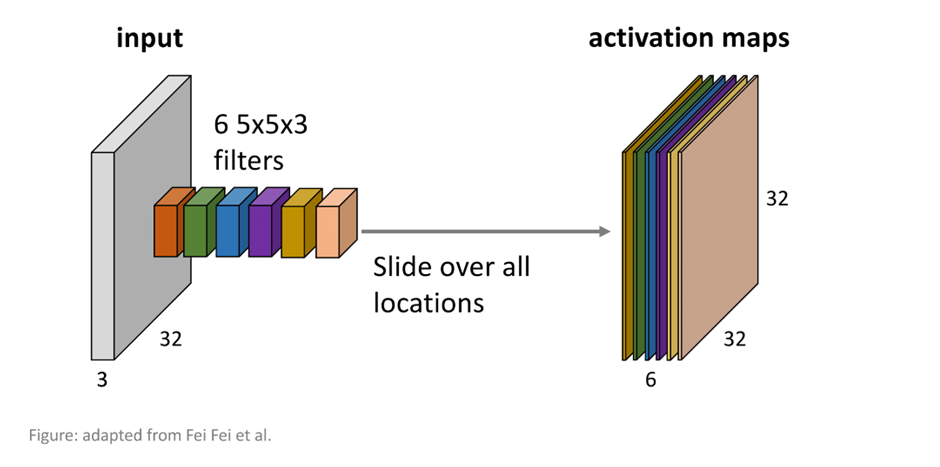
\includegraphics{img/convolution.png}
\end{frame}

\begin{frame}
    \frametitle{Deep Learning}
    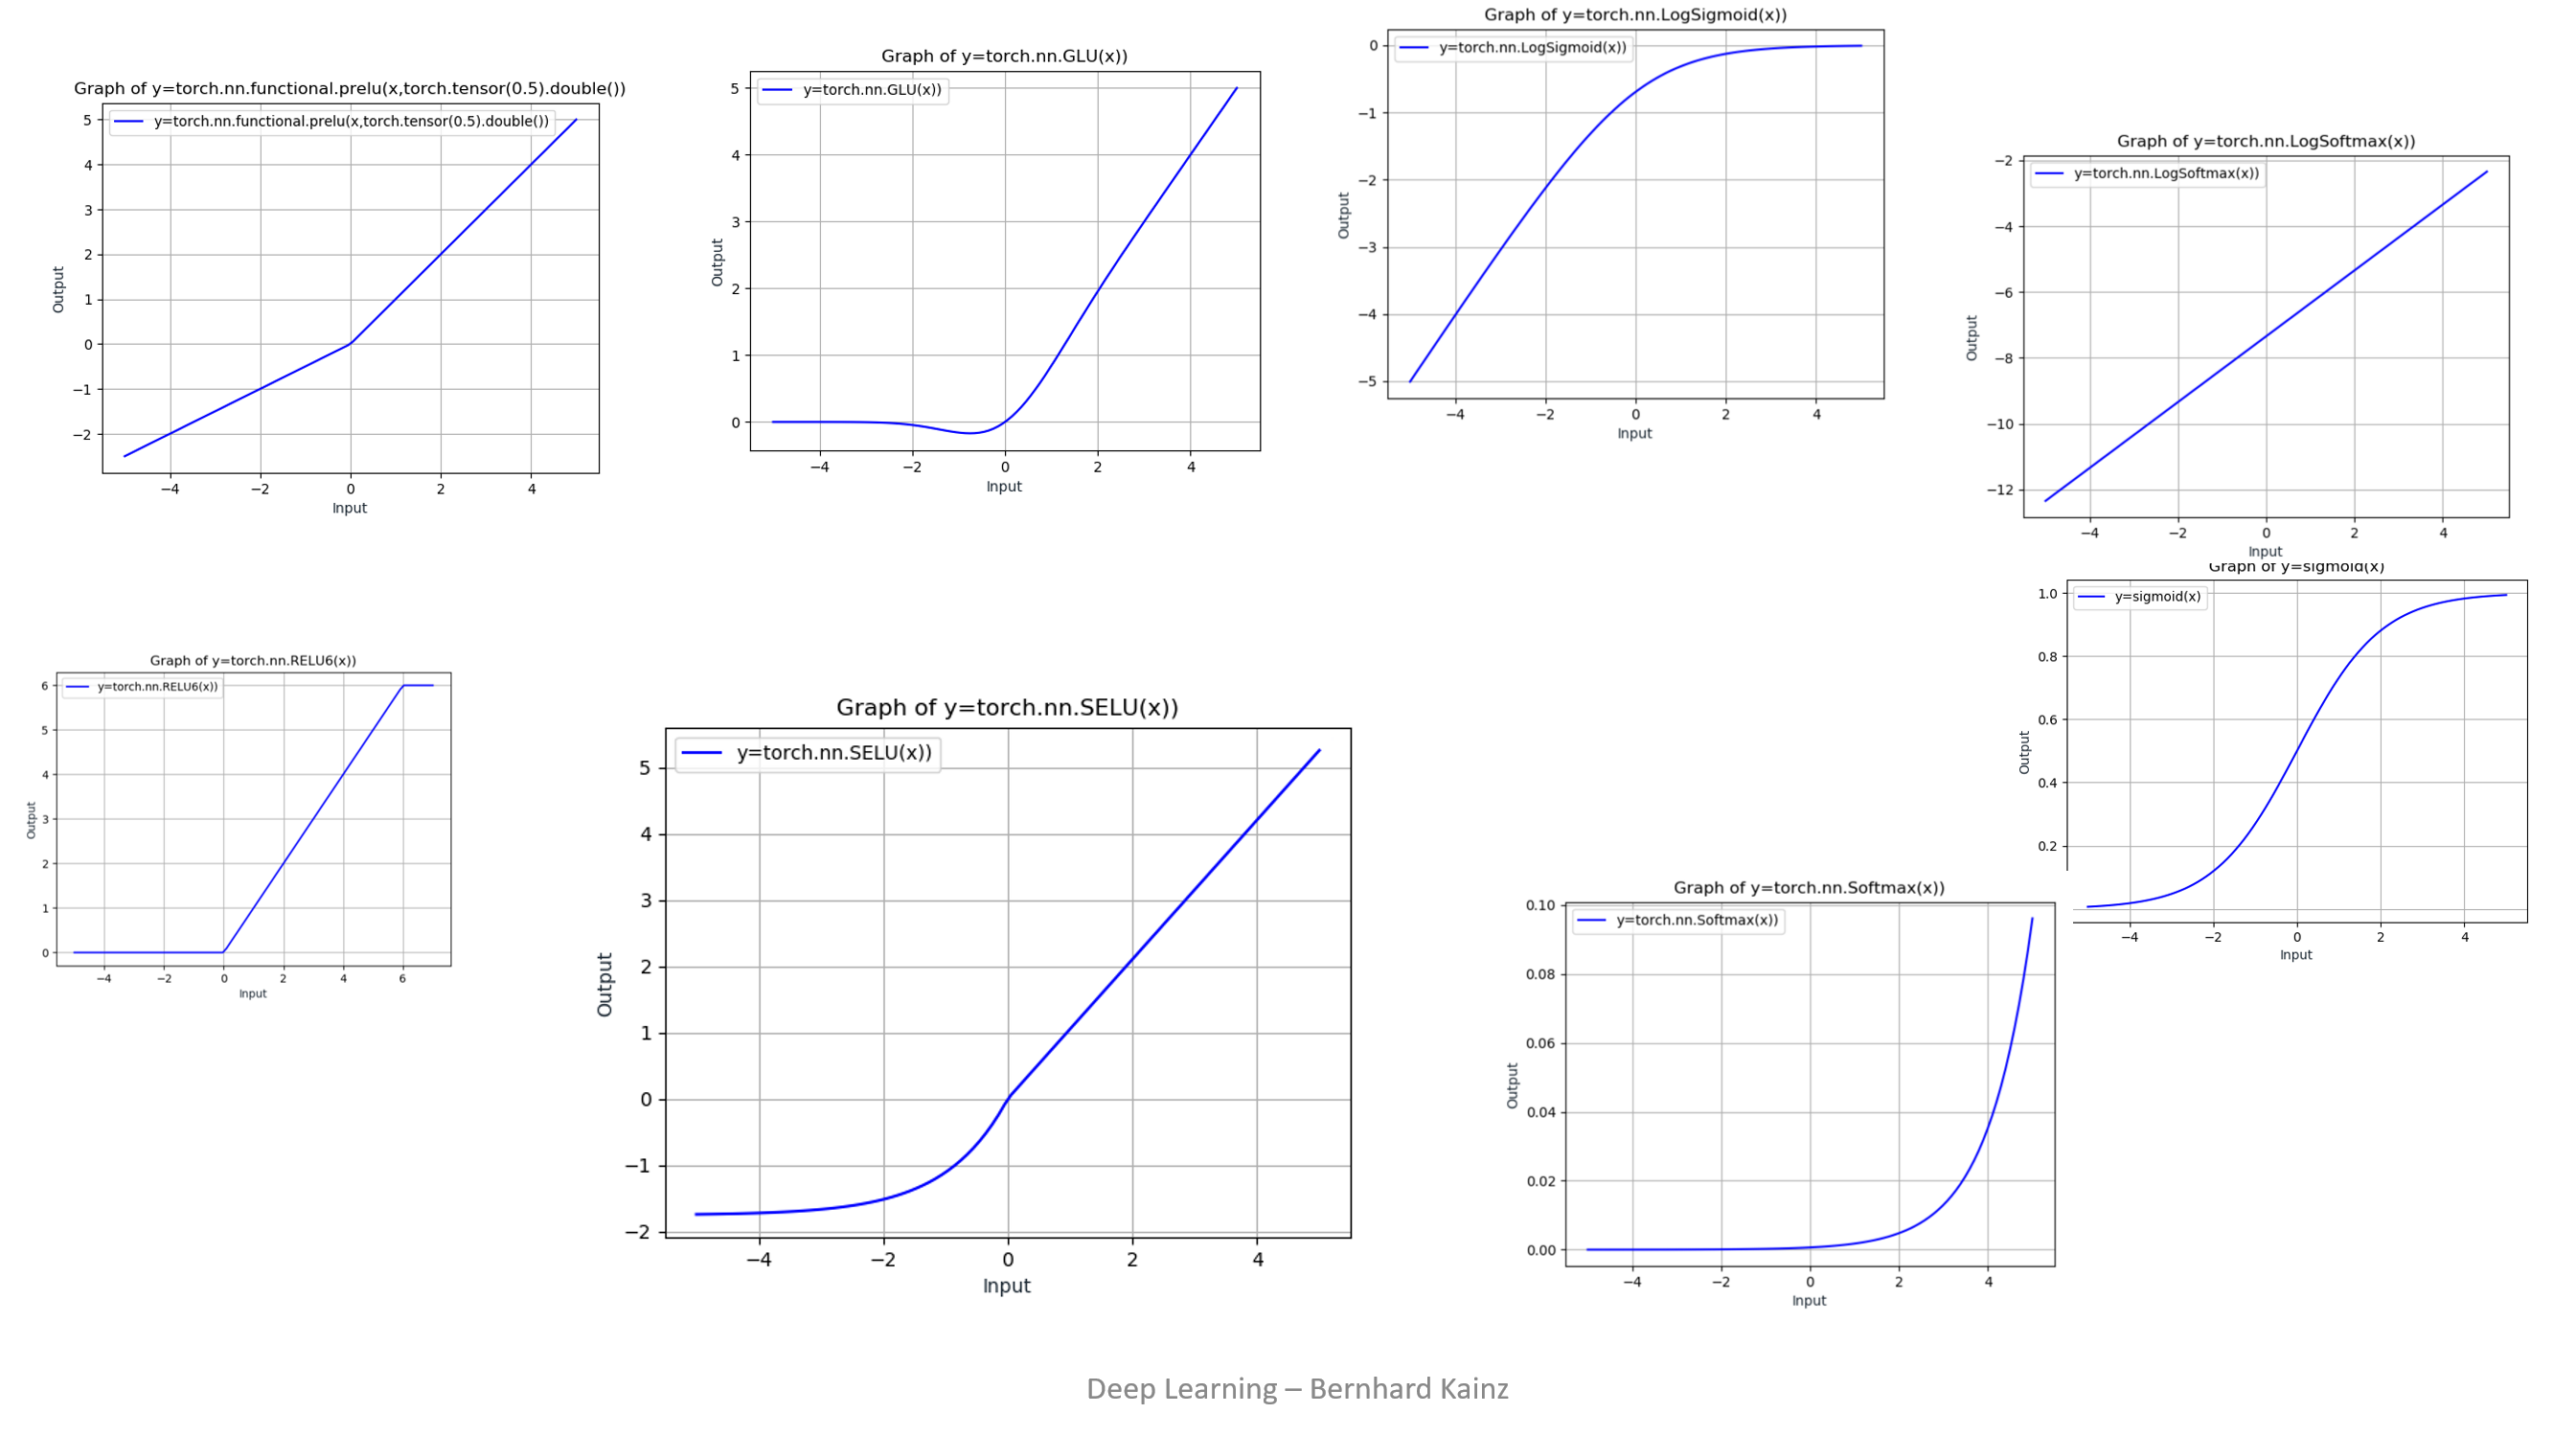
\includegraphics[height=6cm]{img/activation.png}
\end{frame}


\begin{frame}
    \frametitle{Deep Learning}
    \begin{itemize}
        \item \href{https://www.youtube.com/watch?v=81AvQQnpG4Q}{\texttt{Example 1}}
        \end{itemize}
        \begin{center}
    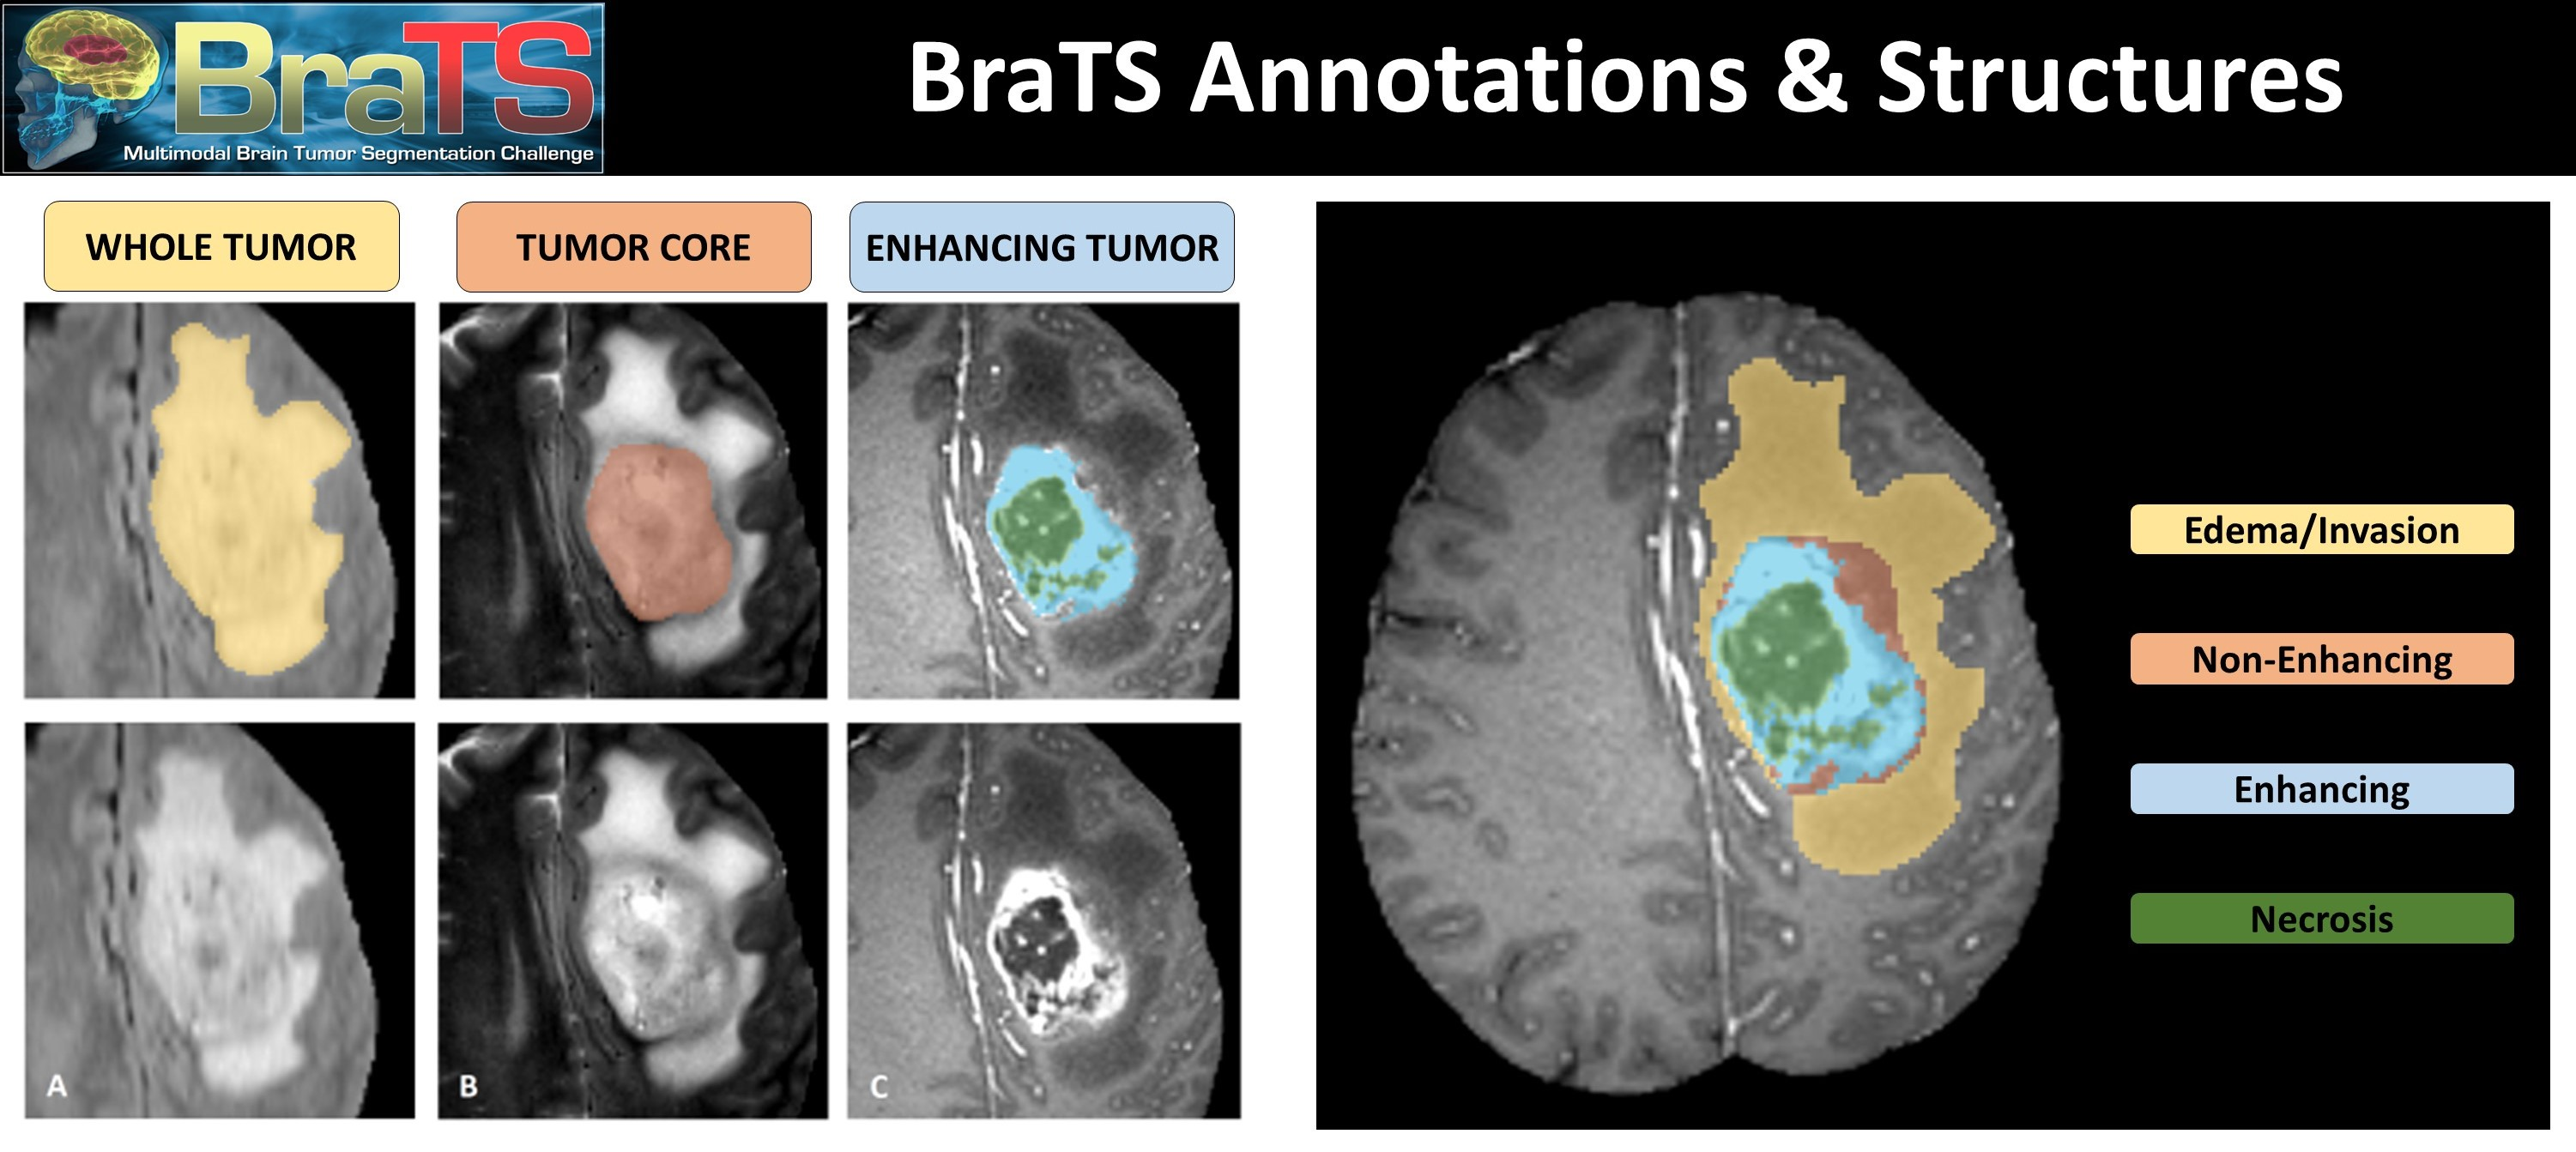
\includegraphics[height=3cm]{img/brats-tumor-subregions.jpg}
    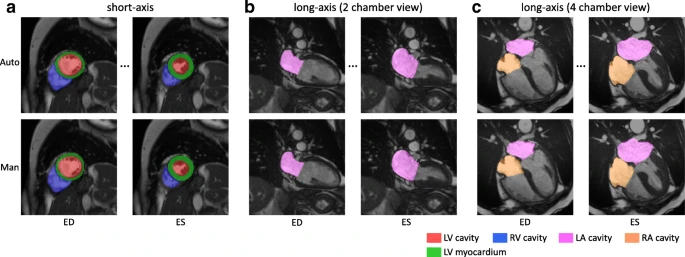
\includegraphics[height=3cm]{img/cardiac.png}
     \end{center}
\end{frame}


\begin{frame}
    \frametitle{Deep Learning}
    \begin{itemize}
        \item \href{https://www.youtube.com/watch?v=4V8V0jF0zFc}{\texttt{Example 2}}
        \end{itemize}
        \begin{center}
    \includegraphics[height=4cm]{img/ultrasound.png}
    \includegraphics[height=4cm]{img/fetal.png}
     \end{center}
\end{frame}



\section{Further Readings}%
\label{sec:further_readings}


\begin{frame}[t]{Further Readings}
    \begin{itemize}
        \item \fullcite{bernecker18}
    \end{itemize}
\end{frame}


\end{document}
